%SAVEDAT= 1453457093
\documentclass[11pt, a4paper]{article} 
\usepackage{slashed,jheppub,multirow,relsize,soul}
\usepackage[normalem]{ulem}
\usepackage{color}

\newcommand{\refeq}[1]{Eq.~(\ref{#1})}
\newcommand{\refeqs}[2]{Eqs.~(\ref{#1})~and~(\ref{#2})}
\newcommand{\refeqss}[3]{Eqs.~(\ref{#1}), (\ref{#2})~and~(\ref{#3})}
\newcommand{\reffig}[1]{Fig.~\ref{#1}}
\newcommand{\reffigs}[2]{Figs.~\ref{#1}~and~\ref{#2}}
\newcommand{\refsec}[1]{Section~\ref{#1}}
\newcommand{\refapp}[1]{Appendix~\ref{#1}}
\newcommand{\reftab}[1]{Table~\ref{#1}}
\newcommand{\refref}[1]{Ref.~\cite{#1}}
\newcommand{\refrefs}[2]{Refs.~\cite{#1}~and~\cite{#2}}

\def\abelian{abelian}
\def\nonabelian{non-abelian}
\def\lagrangian{lagrangian}
\def\eg{\emph{e.g.}}
\def\ie{\emph{i.e.}}
\def\aka{\emph{a.k.a.}}
\def\muboone{MicroBooNE}
\def\minerva{MINER$\nu$A}

%%%%%%% A few editorial macros. %%%%%%%

\newcommand{\lorem}{ \textcolor[rgb]{0.8,0.8,0.8}{Lorem ipsum dolor sit amet, constetur
adipiscing elit, sed do eiusmod tempor incididunt ut labore et dolore magna
aliqua. Ut enim ad minim veniam, quis nostrud exercitation ullamco laboris nisi
ut aliquip ex ea commodo consequat. Duis aute irure dolor in reprehenderit in
voluptate velit esse cillum dolore eu fugiat nulla pariatur. Excepteur sint
occaecat cupidatat non proident, sunt in culpa qui officia deserunt mollit anim
id est laborum.}}

\newcounter{CommentCount}
\setcounter{CommentCount}{1}

\newcommand{\marcom}[2]{\textsuperscript{\textcolor{#1}{\theCommentCount}}\marginpar{\textsuperscript{\textcolor{#1}{\theCommentCount}}\textcolor{#1}{{\small#1: #2}}}\stepcounter{CommentCount}}

\newcommand{\newtext}[2]{\textcolor{#1}{\ul{#2}}}

% Add your own colour down here... 
\definecolor{PB}{rgb}{0.9,0,0}
\definecolor{MARK}{rgb}{0.612, 0.153, 0.69}

%%%%%%%%%%%%%%%%%%%%%%%%%%%%%%%%%%%%%%%


\title{MeV mass sterile neutrino decay at short-baseline neutrino facilities}

\author{One}
\author{Two}
\author{Three}

\affiliation{Institute for Particle Physics Phenomenology, Department of
Physics, Durham University, South Road, Durham DH1 3LE, United Kingdom}

\emailAdd{one@durham.ac.uk}
\emailAdd{two@durham.ac.uk}
\emailAdd{three@durham.ac.uk}

\abstract{
%
We study the sensitivity of the Short-Baseline Neutrino (SBN) program at Fermilab to 
sterile neutrino decay in a variety of models. We show that this experimental complex 
can be expected to extend the known bounds on such decays and comment on the interplay 
between the different beam lines and detector technologies. 
}

\begin{document} 

\maketitle

\section{Introduction}
The Fermilab SBN program \cite{Antonello:2015lea} will comprise of a number of detectors in the Booster Neutrino Beam (BNB): SBND (previously known as LAr1-ND) at 110m from the target, \muboone\ at 470m and ICARUS-T600 at 600m. All three detectors are filled with Liquid Argon (LAr) giving unprecedented reconstruction and particle identification capabilities allowing for significantly lower backgrounds that predecessor technologies. The reconstruction and particle ID capability of LAr technology means the SBN program provides an ideal scenario to study the decay in flight of sterile neutrinos, a job which has traditionally been left for low-mass detectors which had corresponding low beam related backgrounds. 

In addition to events arising from the BNB, the detectors of the SBN complex
will also collect events associated with the NuMI beam, currently being used in
the NO$\nu$A, MINER$\nu$A and MINOS+ experiments. This beam is off-axis with respect to the SBN detectors leading to significant kinematic differences.
\section{Sterile neutrino decay}

Generically, a gauge-singlet fermion will be unobservable by all
non-gravitational means unless it mixes with the active neutrino sector. The
presence of mixing introduces a range of possible observable signatures
depending on the magnitude of the sterile mass and its mixing to the active
sector. 

The most general renormalizable \lagrangian\ extending the SM to include a
single novel gauge-singlet fermion $N$ is given by
%
\begin{align}   \mathcal{L} = \mathcal{L}_\text{SM} +
\overline{N}i\slashed{\partial}N+ \frac{\mu}{2} \overline{N^\text{c}}N  +
\left( y_\alpha\overline{L}_\alpha\tilde{H} N
+\text{h.c.}\right),\label{eq:minimallag} \end{align}
%
where $y_\alpha$ denote Yukawa couplings and $\mu$ a Majorana mass term for
$N$. The extension to multiple new fermions involves promoting $y$ and $\mu$ to
matrices with indices for the new states, but will offer no real
phenomenological difference in the current work.\footnote{The minimal single
$N$ extension does not allow for the observed masses of the neutrinos, as the
mass matrix is rank 1. We assume that an appropriate extension has been
performed to satisfy neutrino oscillation data.} Much work has been done
understanding the phenomenology of novel neutral states, which varies
significantly over their large parameter spaces. An important signal for light
sterile neutrinos are possible observable effects in oscillation experiments,
which could alleviate short-baseline oscillation anomalies; although, no
minimal solution seems to provide a particularly compelling improvement
\cite{}. At larger masses, the neutral particles no longer participate in
oscillation, but these models can generate new signatures at beam dump
experiments \cite{}. At even higher masses, these particles could provide a
natural way to suppress the size of active neutrino masses through the Type I
or III see-saw mechanisms \cite{}. 

Generally speaking, once the neutrinos are massive enough to no longer
oscillate but remain light enough to be produced in terrestrial experiments,
the best way to observe them is through their direct decay into SM particles.
In the minimal \lagrangian\ in \refeq{eq:minimallag}, the only direct couplings
to new sterile fermions are neutrino Higgs interactions. However, these
couplings generate off-diagonal neutrino bilinears below the electroweak
symmetry breaking scale, which leads to mixing between the $4+$ flavours of
neutrinos. Such mixing then introduces production and decay mechanisms of many
kinds for the state $N$ through mass insertion on an active neutrino fermion
line. These decays have been studied extensively in the literature
\cite{Atre} and depend only on the size of neutrino mixing to various
flavours, parameterized by the elements of an extended $4\times4$ PMNS matrix,
%
\[ U_{e4}, \qquad U_{\mu 4} \qquad \text{and} \qquad U_{\tau 4},  \]
%
and the mass of the state $N$ itself. The branching ratios for these decays are
shown in \reffig{fig:branchingratios} as a function of mass for two extremes of
the flavour mixing pattern. On the left, we show the branching ratios if the
new state only mixes with all flavours of active neutrino equally
$U_{e4}=U_{\mu 4}=U_{\tau 4}$, and on the right, when the only mixing with with
$\nu_e$ ($U_{\mu 4}=U_{\tau 4} = 0$). The main effect of the flavour structure
is to forbid certain decays which require certain elements. For example, the
decay of a sterile $N$ into a lepton and a charged pion,
%
\[ N \to l^\pm \pi^\mp,   \]
%
only proceeds if $U_{l4}\neq 0$. This, in turn, affects the possible production
mechanisms for these particles. In a conventional neutrino beam, most neutrinos
are derived from meson decay (or secondary $\mu^\pm$ decays). If $U_{e4}=U_{\mu
4}=0$, such decays with a mass insertion for the sterile neutrino are
impossible for pions or kaons. For this reason, we will mainly focus on mixing
with the first two generations. This parameter space will be probed by working
at higher energies, where the neutral fermions can be produced by decays of
charmed mesons such as $D^\pm$, by the SHiPS experiment \cite{}.
 
\begin{figure}[t]
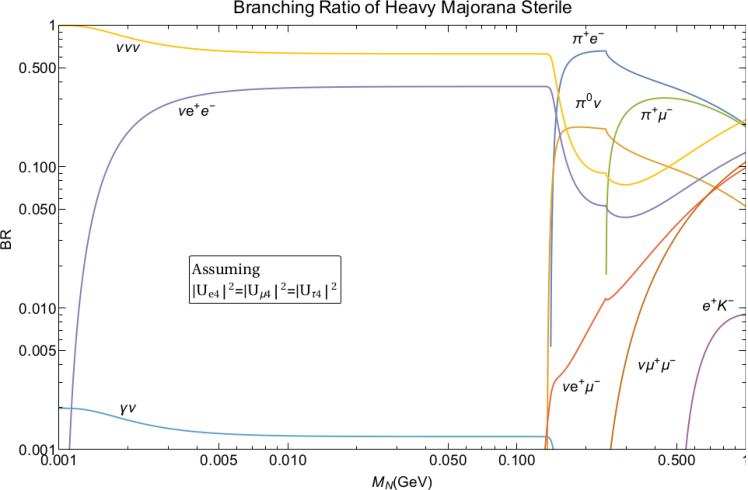
\includegraphics[width=0.49\textwidth]{figures/bounds1.pdf}  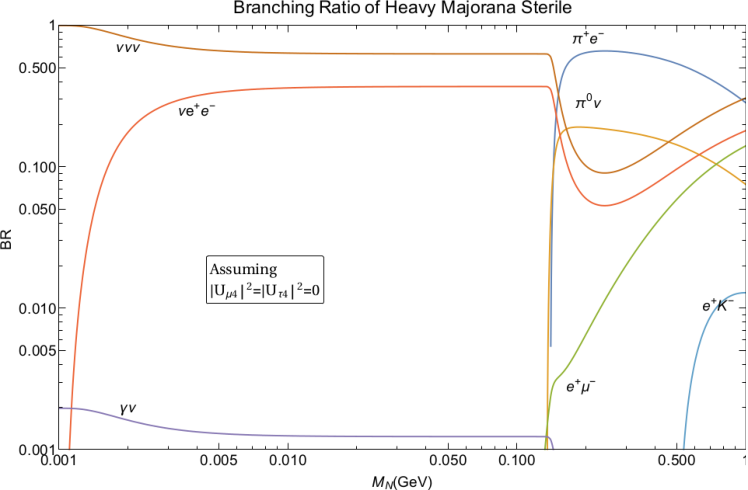
\includegraphics[width=0.49\textwidth]{figures/bounds2.pdf}
\caption{\label{fig:branchingratios}The branching ratios for sterile neutrino decays in the minimal 3 sterile SM extension. The left panel assumes equal mixing with all active flavours, whilst the right panel assumes a flavour hierarchical scheme where only the mixing with $\nu_e$ is important.}
\end{figure}

We highlight four decays in our study, which have the largest branching ratios
of all channels with visible decay products over the mass range $m_\text{s}
\lesssim 1$ GeV. This is based on the minimal sterile extension of the SM
discussed above, but we stress that similar decays can occur in any number of
non-minimal models, where the relationship between decay rate, mass and mixing
can be non-standard. For sterile neutrino masses less than the pion mass, the
dominant visible decay will be into an electron-positron pair as an be seen
from \reffig{fig:branchingratios}. The decay rate for this channel is given by 
%
\[ \Gamma\left(\nu_\text{s}\to \nu_i e^+e^-\right) =
\frac{G_\text{F}^2m_\text{s}^5}{96\pi^3}I(m_\text{s}, U^2).  \]
%
where $I(m_s)$ is an integral. \newtext{PB}{We'll have to decide how to type these things in.}
%
We will base two analyses on this channel, differentiated by the number of
tracks we expect to see. The first event sample will attempt to measure events
where two tracks are resolved, which is expected to have a small background but
favours low-energy events. The second sample studies the converse, where only a
single track can be seen, predominately due to a tightly collimated
$e^+e^-$-pair. In this case we expect a larger background (from anything
producing a single track), but as we will show, we get sizable event numbers in
this channel due to the sterile neutrino's high energy, and a tight cut on the
angular distribution can make it sensitive to sterile decays.

When the mass of the sterile neutrino is greater than the kinematic threshold
for the production of a neutral pion, a new decay dominates
$\nu_\text{s}\to\nu_i \pi^0$. The decay rate for this process is given by
%
\[ \Gamma\left(\nu_\text{s} \to \nu_i \pi^0\right) =
\frac{G_\text{F}^2f_\pi^2m_\text{s}^3}{64\pi}\left[1-\left(\frac{m_\pi}{m_\text{s}}\right)^2\right].
\]

The next channel appears at the kinematic threshold for charged pion production
with a charged lepton. If mixing between the heavy mass state and the electron
neutrino is present, this decay occurs almost immediately after the $\nu\pi^0$
channel opens. However, if this mixing is negligible, there is a the size of
the muon mass before the $\mu^\pm\pi^\mp$ channel opens. As can be seen from
\reffig{fig:branchingratios}, these decays dominate the visible decays when
they are allowed. These decays have a similar scaling behaviour of the decay
rate to the $\nu\pi^0$ channel with an equivalent dependence on the pion
structure constant,
%
\[ \Gamma\left(\nu_\text{s} \to l^\pm\pi^\mp\right) =
\left|U_{l4}\right|^2\frac{2G_\text{F}^2f_\pi^2m_\text{s}^3}{16\pi}I(m_\text{s}).
\]


\lorem\lorem

\section{Simulation details}

We have computed the fluxes and simulated event numbers for each beam and
detector via a custom Monte Carlo program. The program allows efficiency's to
be taken into account due to experimental details of the detector and its
capabilities in a fully correlated way between observables. 

The fluxes from BNB are taken from REF, and we assume no spectral modifications
associated with the altered kinematics of the new sterile neutrino final state.
%
Given the spectral flux of sterile neutrinos in the BNB,
$\mathrm{d}\phi/\mathrm{d}E$, we compute the total number of accepted events in
channel ``$\text{c}$'' via the following summation,
%
\[ N_\text{c} = \sum_{i} \left .
\frac{\mathrm{d}\phi}{\mathrm{d}E}\right|_{E_i} P_\text{D}\left(E_i\right)
W_\text{c}\left(E_i\right),  \]
%
where $P_\text{D}(E)$ is the probability for a sterile of that energy to reach
and then decay inside the detector labelled $\text{D}$. The simplest
approximation is to ignore all geometric effects, so that every particle
travels exactly along the direction of the beam line, which gives the following
probability 
%
\[ P_\text{D}\left(E\right) = e^{-\frac{\Gamma_\text{T}L}{\gamma\beta}}\left(
1-
e^{-\frac{\Gamma_\text{T}\lambda}{\gamma\beta}}\right)\frac{\Gamma_\text{c}}{\Gamma_\text{T}},
\label{eq:prob}
\]
%
where $\Gamma_\text{T}$ ($\Gamma_\text{c}$) denotes the rest-frame total decay
width (decay width into channel $\text{c}$), $m$ the mass of the sterile
neutrino, and $L$ ($\lambda$) the distance to (width of) the detector. The
combination $\gamma\beta$ is the usual special relativistic function of
velocities of the parent particle and provides the sole energy dependence of
the expression
%
\[   \frac{1}{\gamma\beta} \equiv \frac{m}{\sqrt{E^2-m^2}}. \]
%
As we are exploring a large parameter space, often this expression takes a
simplified form depending on the size of $\Gamma_\text{T}\lambda/\gamma\beta$:
%
\begin{align*} 
%
\Gamma_\text{T}\lambda \ll 1\qquad&\qquad P_\text{D} \approx
e^{-\frac{\Gamma_\text{T}L}{\gamma\beta}}\frac{\Gamma_\text{c}\lambda}{\gamma\beta}
+ \mathcal{O}\left(\Gamma_\text{T}^2\lambda^2\right),\\ 
%
\Gamma_\text{T}\lambda \gg 1\qquad&\qquad P_\text{D} \approx
e^{-\frac{\Gamma_\text{T}L}{\gamma\beta}}\frac{\Gamma_\text{c}}{\Gamma_\text{T}}
+ \mathcal{O}\left(\frac{1}{\Gamma_\text{T}\lambda}\right), 
%
\end{align*}
%
where the rate for slowly decaying particles can be seen to grow with detector
size until a width of $\lambda\sim\Gamma_\text{c}^{-1}$ where longer detectors
make no difference, as most steriles decay within a few decay lengths and
therefore we see a fixed fraction of the total events in our channel of interest. 
We will comment on how the three detectors of the SBN complex can use the 
dependence on $E$ and $L$ in these expressions to enhance their sensitivity in 
Section ??.

%
Finally, the function $W_\text{c}(E)$ is a weighting factor which accounts for
all effects which reduce the number of events in the sample: for example,
analysis cuts or detector performance effects.
%
To compute these factors, we run a Monte Carlo simulation of the decays for a
large number of sample events with a given energy. Each sterile event is
associated with a decay of type $\text{c}$. We then apply experimental analysis
cuts to the decays based on our assumptions about the detector's capabilities
and backgrounds, to produce a spectrum representing the final event sample. The
percentage of accepted events defines the weight factor for that energy.

We also work spectrally producing the expected distributions of observed
events. This can be used to suggest improved analysis cuts based on the
interplay between the three detectors of the SBN complex. We return to this in
section II.

\subsection{Sterile neutrino fluxes}

To leading order in the mass of the sterile neutrino over the pion, the fluxes
for the $\nu_\text{s}$ will be a rescaling of the fluxes for the active
neutrinos.  We take these fluxes as our input and scale them by the appropriate mixing $U_{\alpha 4}$, with an additional kinematic factor to take into account the helicity un-suppression of $\pi^+ \rightarrow e^+\nu_s$ for massive $\nu_s \gg m_e$, such that for a sterile produced from the decay of a meson M
\[
	\phi_{\nu_s} \approx \phi_{\nu_\alpha} \vert U_{\alpha 4}\vert^2 \frac{\Gamma(M \rightarrow \nu_s \alpha)}{\Gamma(M\rightarrow \nu_\alpha \alpha)}.
\]
This kinematic effect for the pion and kaon, the only mesons produced in large numbers in the BNB beam, is shown below in figure \ref{fig:flux_enhancement}. We only consider steriles below the kinematic threshold of the kaon, as although there is a small component of heavier mesons such as the D meson which could produce heavier states, they are produced in very small numbers due to the relatively low energy protons of the NB beam. 

\begin{figure}[t]
\center
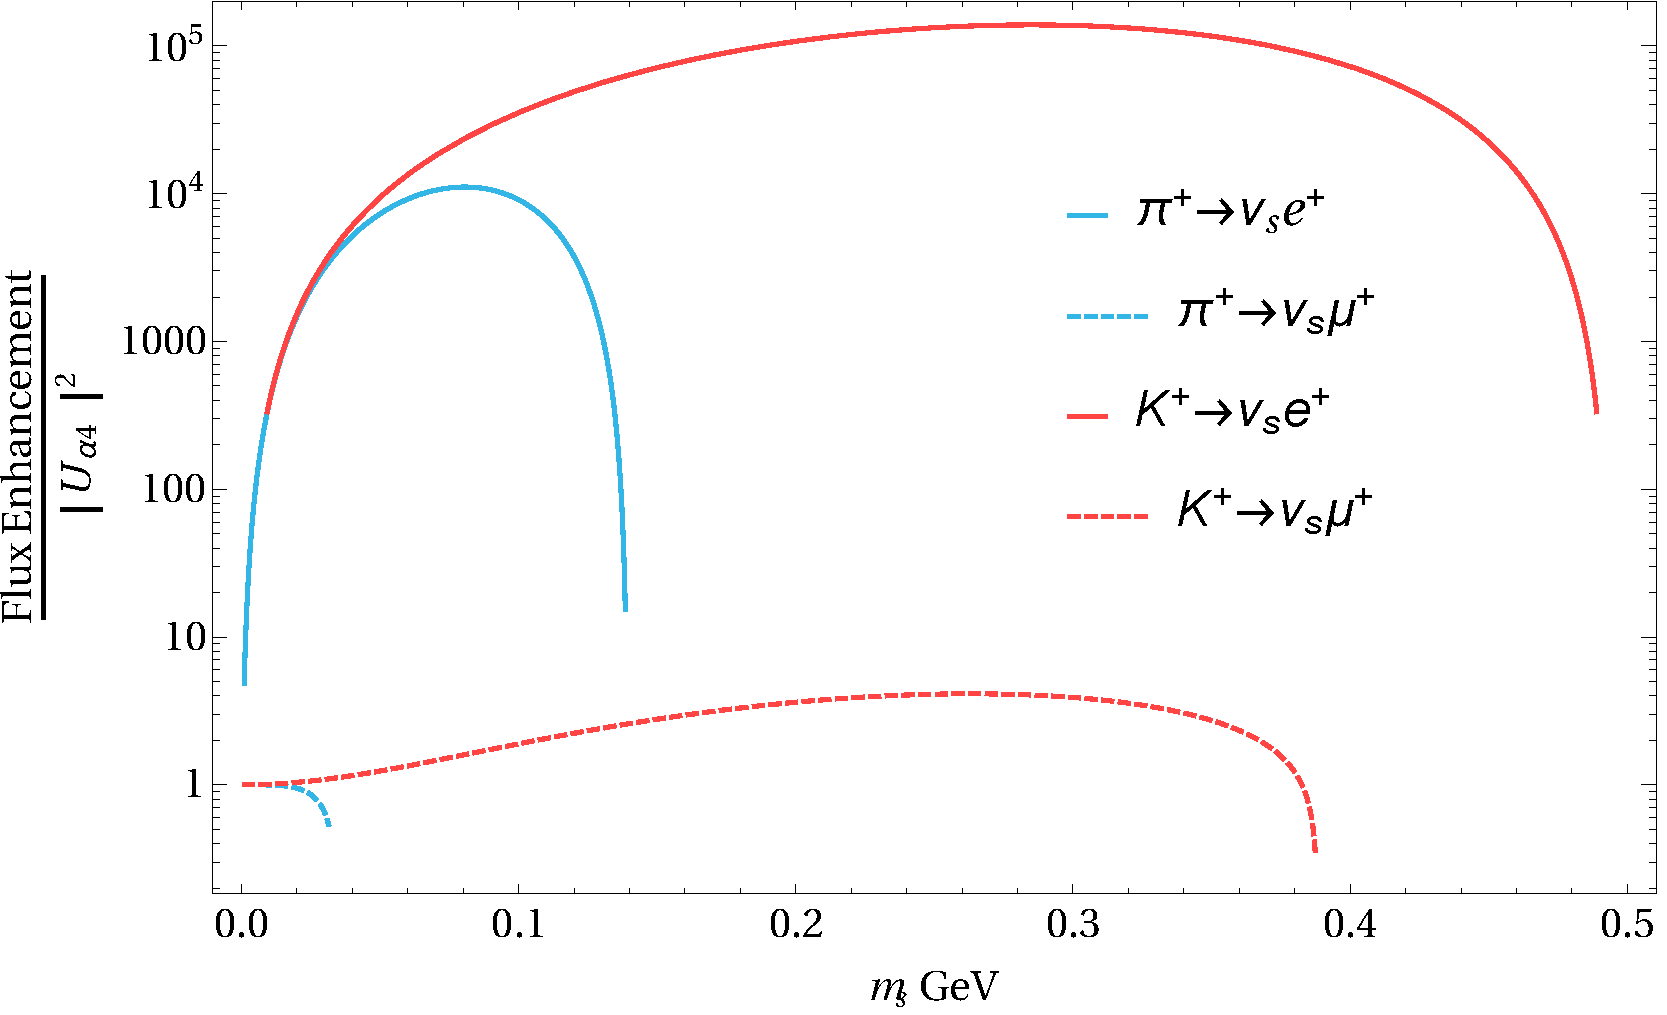
\includegraphics[width=0.6\textwidth]{figures/BNB_flux_enhancement.pdf}

\caption{\label{fig:flux_enhancement} Kinematic enhancements of the sterile flux, for the four production channels available for steriles in the BNB beam. There is little effect when mixing with muons alone, as the muon is heavy enough to remove the helicity suppression that usually kills the $\pi\rightarrow e \nu$ channels. This factor of up to $10^5$ enhancement more than compensates for the significantly smaller flux of $\nu_e$ always inherent in the BNB beam.}

\end{figure}



%
\newtext{PB}{Can we add a figure of the fluxes? Perhaps some comment on how we
are modelling them. This is all finished, right? (Unless we start doing
something wild with the NuMI fluxes).}
%
\lorem\lorem 

\subsection{Detector modelling and analysis cuts}

To compute the weighting factors $W_\text{c}$, we generate a large number of
Monte Carlo events of the decay that we are interested in and remove those
events which fail a series of cuts. These cuts are designed to reflect both
genuine analysis cuts designed to enhance the signal to background ratio (for
example, choosing events with energies within certain ranges), as well as cuts
which provide a basic model of detector effects and limitations (for example,
discarding events that wouldn't be reconstructed correctly, \eg\ those with
overlapping tracks in a two particle final state).

We summarize our cuts in \reftab{tab:cuts}.
%
\begin{table}[t]
\centering
\begin{tabular}{ l | l | l}
Signal & Constraint & Value \\
\hline\hline
 \multirow{4}{*}{$e^+ e^-$ (two tracks)} & low-energy thresh. & $50$ MeV\\
 \cline{2-3}
 & foreshortened angular separation & $>5^\circ$ \\
 \cline{2-3}
 & energy ratio $E_\text{low}/E_\text{high}$ & $>0.1$\\
 \cline{2-3}
 & angle? & $100\%$\\
\cline{1-3}
 \multirow{4}{*}{$e^+ e^-$ (single track)} & low-energy thresh. & $50$ MeV\\
 \cline{2-3}
 & foreshortened angular separation & $<5^\circ$ \\
 \cline{2-3}
 & energy ratio $E_\text{low}/E_\text{high}$ & $<0.1$\\
 \cline{2-3}
 & angle? & $100\%$\\
\cline{1-3}
 \multirow{3}{*}{$\pi^+e^-(\pi^-e^+)$} & low-energy thresh. & $10$ MeV\\
 \cline{2-3}
 & energy ratio $E_e/E_\pi$ & $>0.1$\\
 \cline{2-3}
 & angle? & $100\%$\\
\cline{1-3}
 \multirow{3}{*}{$\pi^+\mu^-(\pi^-\mu^+)$} & low-energy thresh. & $10$ MeV\\
\cline{2-3}
 & energy ratio $E_\mu/E_\pi$ & $>0.1$\\
\cline{2-3}
 & angle? & $100\%$\\
\end{tabular}
\caption{\label{tab:cuts}Detector cuts as modelled in our simulation.}
\end{table}
\newpage
\newpage

\subsection{Signal distributions}

\newtext{PB}{We can compute all types of kinematic distributions to talk about
cuts.} See \reffig{fig:ang_sep_E_total}.

\begin{figure}[t]
\center
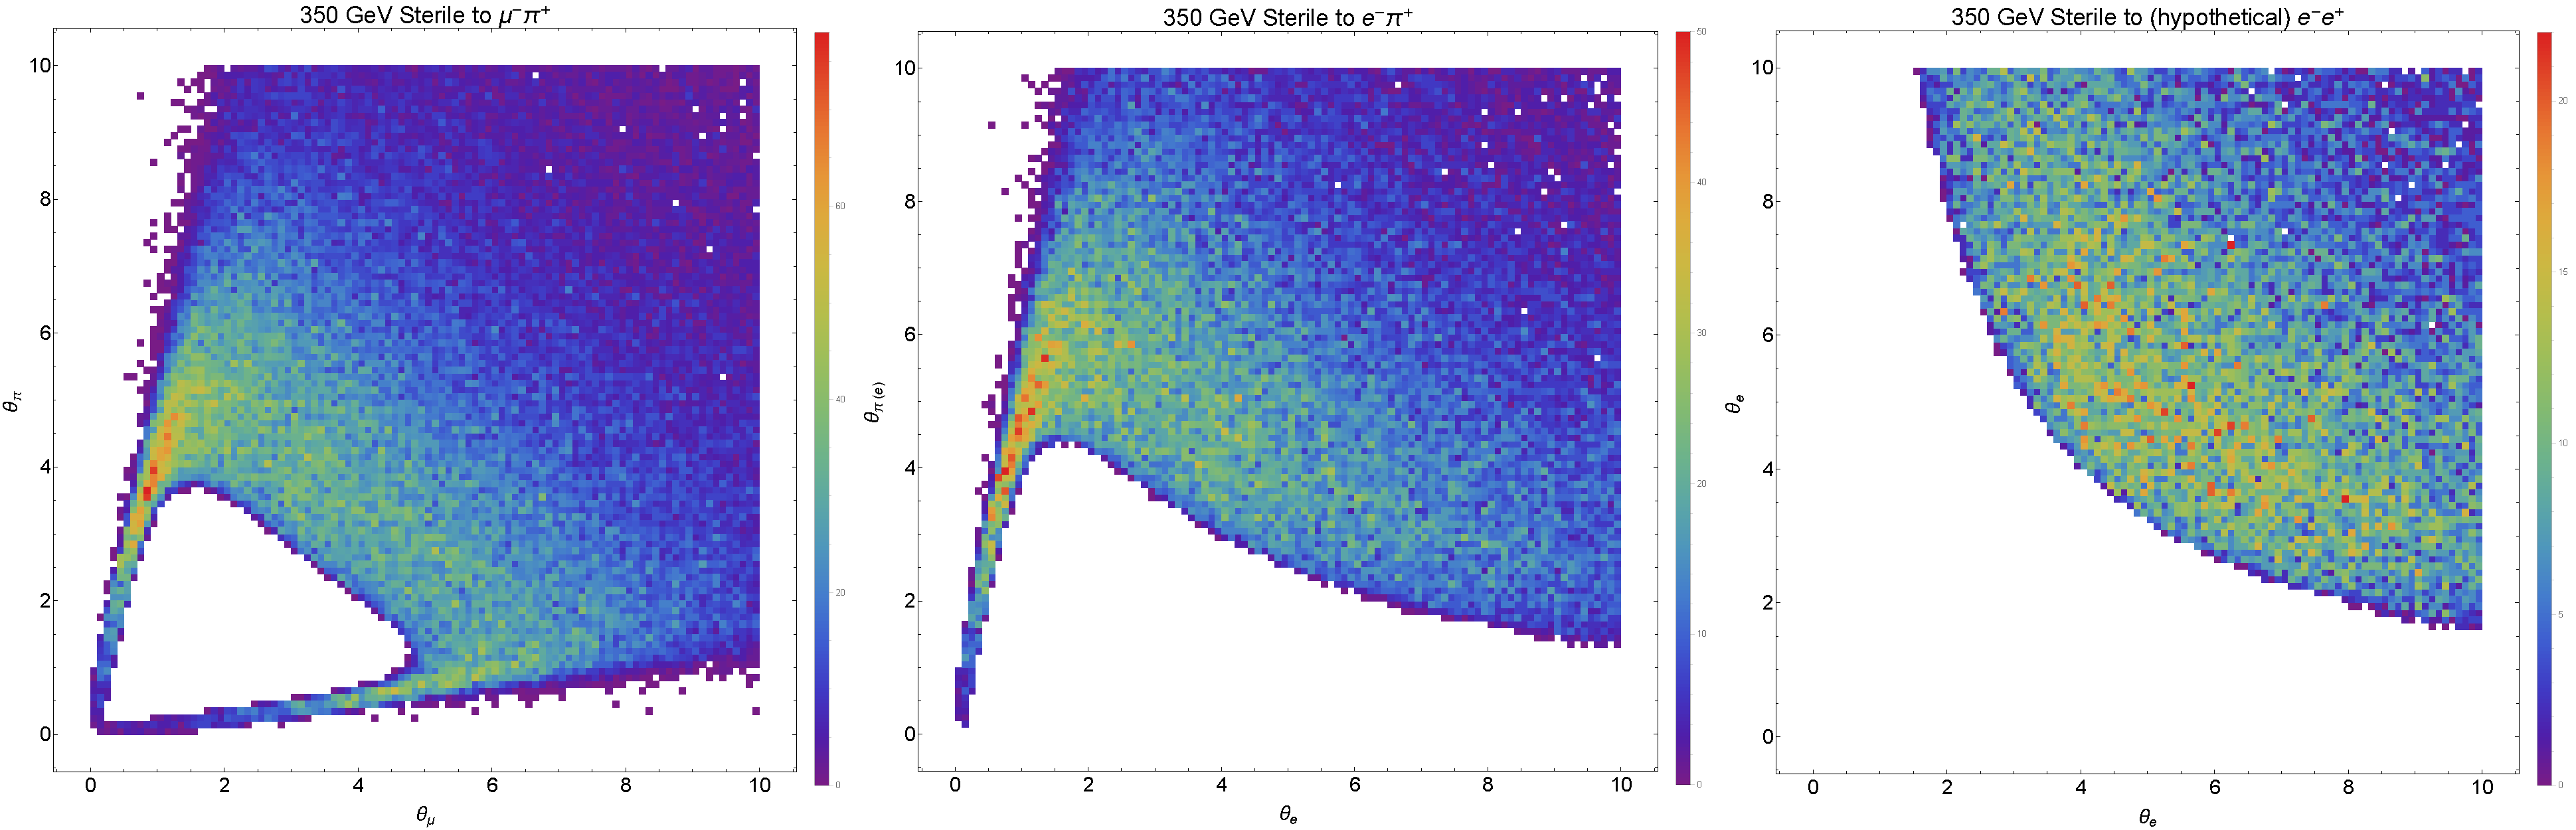
\includegraphics[width=1.0\textwidth,clip,trim=0 0 0 0]{figures/all_dist.pdf}

\caption{\label{fig:all_dist} The angular distributions of the lepton and pion pair from sterile neutrino decay in flight at $\mu$BooNE. }

\end{figure}


\begin{figure}[t]
\center
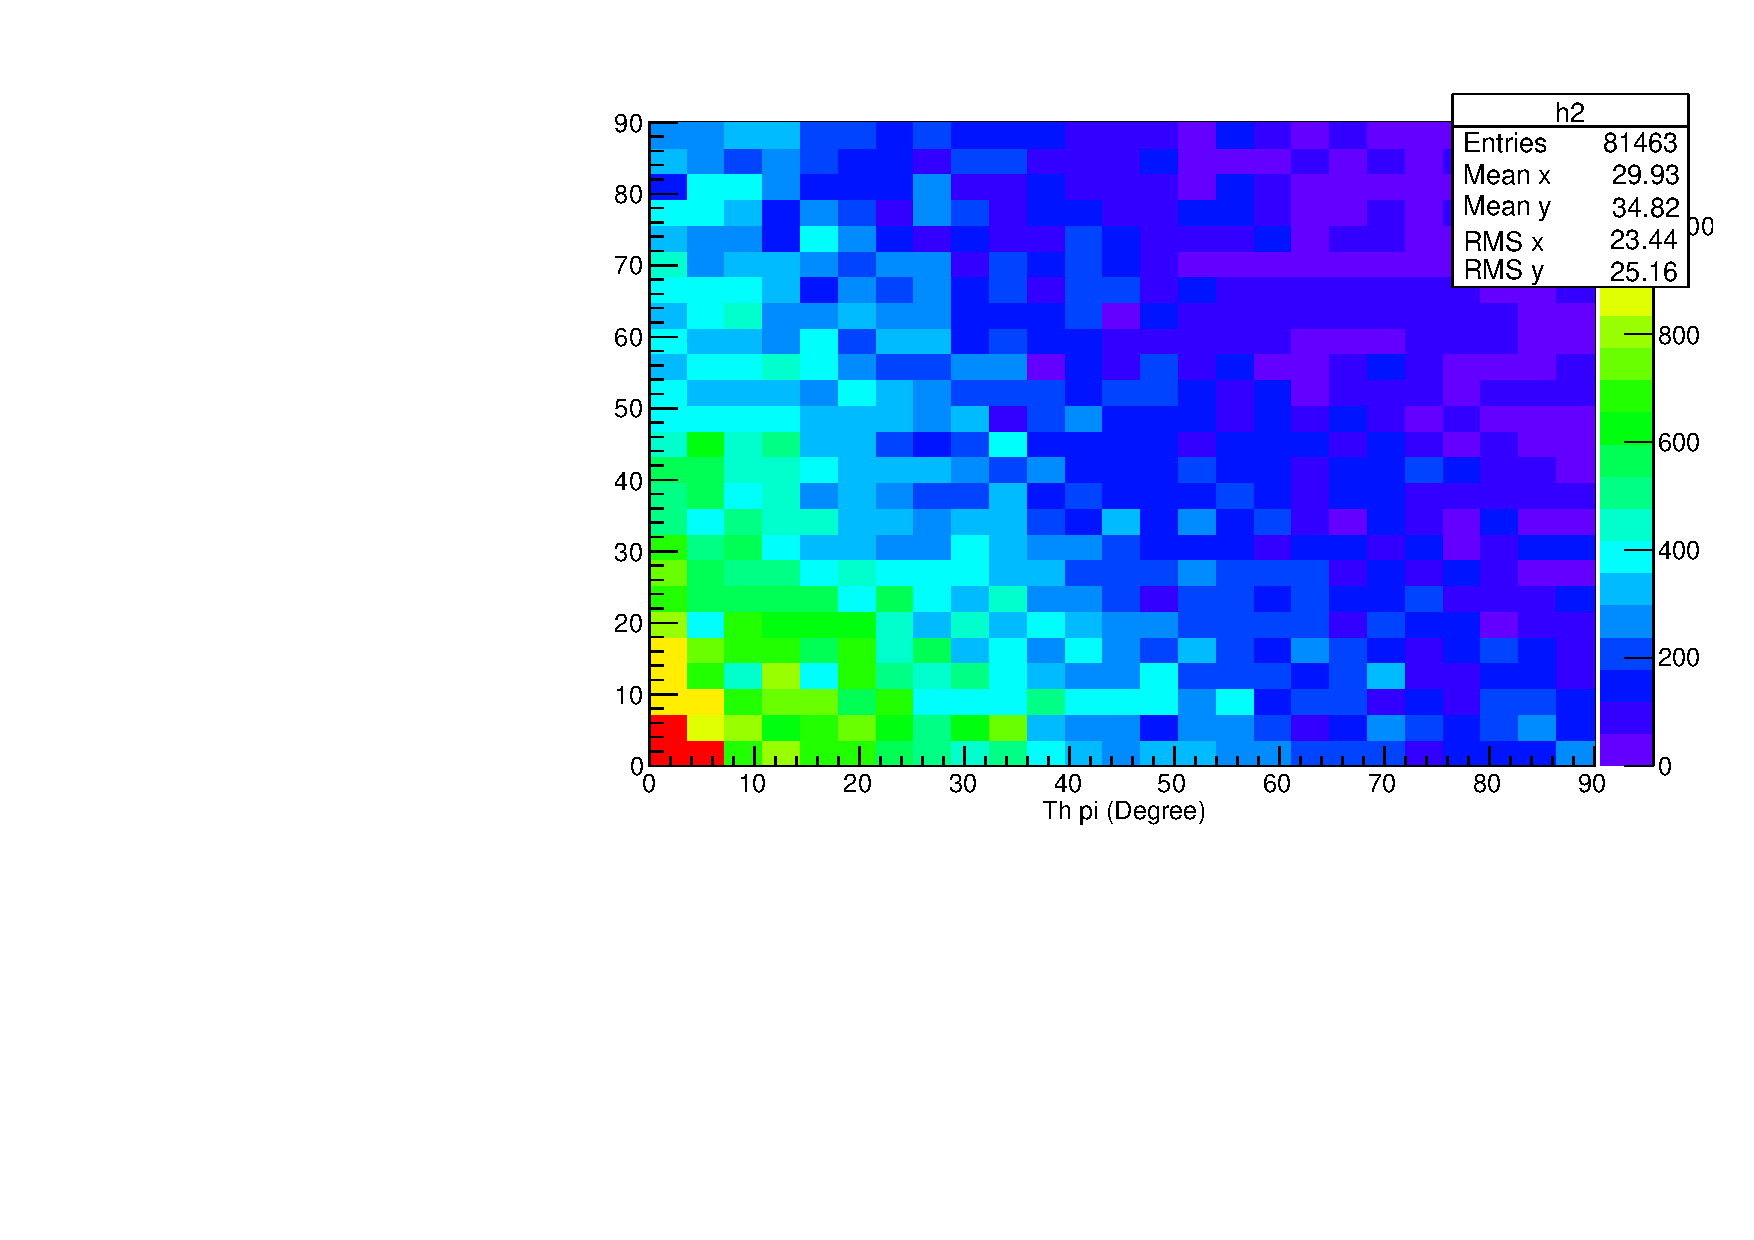
\includegraphics[width=0.6\textwidth,clip,trim=0 0 0 0]{figures/angdist_bkg.pdf}

\caption{\label{fig:angdist_bkg} The angular distributions of the beam driven CC $\nu_\mu N \rightarrow N^\prime \mu^- \pi^+$, the predominant background to the $\nu_N \rightarrow \mu^- \pi^+$ decay search. }

\end{figure}



\begin{figure}[t]
\center
\includegraphics[width=1.0\textwidth,clip,trim=0 0 0 0]{figures/ang_sep_E_total_plot.pdf}

\caption{\label{fig:ang_sep_E_total}The distribution of total energy deposited in an $e^+e^-$ pair from sterile neutrino decay in flight at $\mu$BooNE against the apparent angular separation of the two particles.}

\end{figure}



\newpage
\subsection{Background modelling}

\begin{table}[t]
\centering
\begin{tabular}{ l | l | l| l | l}
	Signal Channel & Main Background & Events @ SBND & MicroBooNE & Icarus \\
\hline\hline
\multirow{1}{*}{$\mu^\pm \pi^mp$} & CC: $\nu_\mu  \rightarrow \mu \pi + \text{``nucleons''} $ & 1,161,610  & 101,123 & 165,933\\
\multirow{1}{*}{$ e^\pm \pi^\mp$} & CC: $\nu_e  \rightarrow e \pi + \text{``nucleons''} $ & 8,200  & 713 & 1,171\\
\multirow{1}{*}{$ \nu_\alpha \pi^0$} & NC: $\nu_\mu  \rightarrow \nu_\mu \pi^0 + \text{``nucleons''} $ &  358,443 & 31,204 & 51,202\\
 \multirow{1}{*}{$ e^+e^- \text{ (Distinguishable)} $} & CC: $\nu_e  \rightarrow e \gamma + \text{``nucleons''} $ &  --- & --- & ---\\
  \multirow{1}{*}{$ e^+ e^- \text{ (Photon-like)}$} & NC: $\nu_\mu  \rightarrow \nu_\mu \gamma $ &  --- & --- & ---\\
 \hline \hline

\end{tabular}
\caption{\label{tab:Rates} A summary of the main sources of backgrounds for each channel studied, before spectral and particle ID cuts are applied. }
\end{table}


For each channel studied in this analysis, we have implemented a model of the dominant processes contributing to the backgrounds. The properties of these backgrounds will motivate our cuts. We will discuss the details of the modelling that we have performed in a channel-by-channel basis. The number of expected background events before cuts is summarized in Table (\ref{tab:Rates}) above. Here we focus on beam driven backgrounds, with the assumption that cosmogenic backgrounds are significantly less of an issue via timing and directional cuts. 


\subsubsection{$\nu_N \rightarrow \mu^\pm \pi^\mp$ }

Pions produced inside the SBN LAr detectors will quickly decay into muons, which, if of low enough energy,
subsequently decay into Michel electrons. We can expect this chain of decays to
be well reconstructed in liquid argon if the pion and muon are contained, and the dominant backgrounds to the
sterile decays we are interested in will be genuine $\pi$-lepton production
associated with the neutrino beam. So-called CC1$\pi^+$ events are defined as
the associated production of a charged pion from the standard CC process which
produces a lepton. This can happen by resonant production, where a nucleon is
excited into an unstable state, for example into a $\Delta$, and the following
decay produces a nucleon and a pion. Such decays are characterized by a
a relatively isotropic spectrum due to the relatively mild boost of the resonant state
\cite{Rein:1982pf}. There may be one or more protons or neutrons also emitted in these scattering events. 

Another contribution to the cross-section is from coherent
scattering, where the neutrino scatters from the whole nucleus 
%
\[   \nu_l + A \to l^- + A + \pi^+ \qquad\text{or}\qquad \overline{\nu}_l + A
\to l^+ + A + \pi^-. \]
%
These interactions tend to produce more forward decay products and will be another significant source of backgrounds. Cross-sections for these processes have been studied in MiniBooNE \cite{Wascko:2006tx} and \minerva\ \cite{Eberly:2014mra} and cross-sections appear to agree with Monte Carlo calculations based on the Rein-Sehgal model \cite{Rein:2006di, Rein:1982pf}. Such a low $Q^2$ process tends to favour daughter pions and muons that are forward going, kinematically very similar to decays in flight, as well as no observable nuclear activity. ArgoNeut analysis estimates the approximate number of events, for similar liquid argon technology to $\mu$BooNE \cite{Acciarri:2014eit}. For low energy neutrino beams, no events have been observed thus far, see SciBooNE \cite{Tanaka:2009ag} and high energy event rates are in accordance with what is expected, see NOMAD \cite{Kullenberg:2009pu}.

\subsubsection{$\nu_N \rightarrow e^\pm \pi^\mp$ }
If there is a non-zero $U_{e4}$ then the decay to electron and charged pion opens up when $m_\pi +m_e \leq m_N \leq m_K$. The expected numbers of $e \pi$ events in the SBN detectors is significantly smaller than that of the $\mu \pi$ channel, as the fraction of inherent $\nu_e$ in the BNB beam is of $\mathcal{O}(1\%)$ level. However, there will be additional backgrounds to the $e \pi$ channel from the dominant $\nu_\mu$ beam. CC $\nu_\mu$ events which contain an additional photon $(\mu+\gamma)$ could be mis-identified as an $(\pi e)$ decay provided the muon is of low energy and has a short track length.

\subsubsection{$\nu_N \rightarrow \nu_\alpha e^+ e^-$ }
A sufficiently boosted, and thus overlapping such that shower separation is not possible, $e^+e^-$ pair is indistinguishable from a converted photon in a LAr detector. The rate of energy loss of the $e^+e^-$, $dE\/dx$, would also match up with that of a pair-converted photon, meaning separation is near impossible.  As such any process producing a lone stray photon is a possible source of backgrounds for this channel. The predominant source of this is the SBN detectors is the decay of a neutral pion in which a single photon is not resolved. This background, however, is relatively isotropic in distribution, in stark contrast to the very forward signal. We define all $e^+e^-$ pairs in which the angle of separation between them $\leq 1^\circ$\cite{Spitz:2011wba}, as unresolvable and thus ``overlapping''. The majority of such overlapping events originate from low mass parent steriles, $\leq 50$ MeV.\\
	

The opposite scenario also arises, in which both daughter electron have a well defined large separation and can cleanly be identified as two distinct single electron electromagnetic showers. Here the majority background is CC $\nu_e$ interactions in which the electron is accompanied by a photon which is mis-identified as an electron, or a NC produced $\pi^0$ decay in which both of the underlying photons are mis-identified as electrons. As there is little standard processes what produce high energy distinct $e^+e^-$ pairs, the backgrounds usually require mis-identification of one or more particles, combined with the requirement that there is little or no hadronic activity, means that the expected rates are significantly lower than that of the photon-like $e^+e^-$ sample.

\subsubsection{$\nu_N \rightarrow \pi^0 \nu_\alpha$}
Although a sub-dominant decay mode when steriles mix with electrons alone, when one considers non-zero $\vert U_{\mu4}\vert^2$ the branching ratio of $\nu_s \rightarrow \nu_\mu \pi^0$ becomes dominant for a mass window $\approx 140 \rightarrow 240$ MeV. Single neutral pions are produced in great numbers at the three SBN facilities, so the lack of any nuclear recoil is crucial in eliminating the incoherent neutral pion production background. The NC coherent pion production, however, does not contain any nuclear tracks and so will be an irreducible background for this channel, up to spectral kinematics.

\subsubsection{Non-Beam related backgrounds}
Cosmogenic backgrounds are expected to be significantly smaller in comparison to beam related backgrounds. In the case of cosmic muons, Icarus expects to see approximately $2.5 \times 10^{6}$ cosmic events in the 211 second beam spill, and are reduced to approximately 5 events expected after utilizing the spill structure, scintillation light patterns and cuts on $\frac{d E}{d x}$ \cite{Antonello:2015lea}. Similarly for cosmic backgrounds to electron (photon) like signals 170 (146), 136 (88) and 498 (154) are expected at SBND, MicroBooNE and Icarus respectively, however, they are predominately in the low energy bins, $< 0.5$ GeV. Alongside this impressive cosmic rejection, our signal events are focused heavily along the beamline, hence we do not expect cosmics to be a major source of background to any channel are are not included in this analysis. Total flux uncertainties have little effect on the resultant sensitivities as shifts affects both signal and beam driven background equally. Cross-sectional uncertainties, however, have the potential to modify all beam related backgrounds while leaving the decay in flight signal unchanged and thus are an unavoidable source of uncertainty.


As can be seen in Table \ref{tab:Rates}, he total numbers of background events expected in each channel can very large, up to $10^6$ $\mu+\pi$ evens in SBND. However, these numbers do not take any spectral or kinematic information into account. In order to provide a more accurate estimation we perform a full Monte-Carlo analysis of the expected backgrounds using the neutrino event generator GENIE. This provides us with generator level information about the kinematics of the majority of the beam-driven backgrounds. Energy and angular smearing is then implemented to allow for approximate estimates of the effect of detector performance to the level necessary for this analysis, without the need for a full GEANT detector simulation. Energies are smeared according to a Gaussian distribution around their true MC energies, with a relative variance $\sigma_E/E = \xi/ \sqrt(E) $, where $\xi$ is a detector dependant resolution. For this study we take the energy resolution for EM showers, muons and protons to be 15\%, 6\% and a conservative 20\% respectively.

For the hadronic modes, $\nu_N \rightarrow e^\pm \pi^\mp$ and $\nu_N \rightarrow \mu^\pm \pi^\mp$, the majority of background rejection capability comes from four kinetic cuts. Exact efficiency's are given for a reference decaying 0.350 GeV sterile neutrino in MicroBooNE.

\begin{enumerate}
	\item {\bf Hadronic Activity.} Of up most importance to distinguishing signal and background is the identification of a scattering vertex. Any hadronic activity localized at the leptonic beginning of the lepton track is a smoking gun signal for beam related scattering from deep-inelastic or quasi-elastic scattering. Therefore any event containing one or more reconstructed protons or additional hadrons is rejected outright. For counting this proton multiplicity we assume an detection threshold of 21 MeV on proton kinetic energy in liquid Argon, after smearing.
	\item {\bf Forwardness Cut.} Both the lepton and pion produced from such heavy sterile decays tend to both be very forward in the lab frame. In contrast, a large fraction of scattering backgrounds are significantly more isotropic in their distribution. Therefore a cut on both lepton and pion emission angles to be within $20^\circ$ of the beamline is applied.
	\item {\bf Invariant Mass Cut.} The invariant mass of the lepton pion pair, $M_{l^\pm \pi^\mp}^2=m_l^2+m_{p^\pm}^2+ 2(E_l E_\pi - |P_l||P_\pi|\cos\theta_\text{sep})$, will sum to that of the the parent sterile (within detector resolution), where as the background is expected form a dropping continuum spectra. We therefore cut on any events whose invariant mass is outside a 20 MeV window surrounding the parent sterile mass.
	\item {\bf Pion Energy Cut.} Finally sterile decays in flight tends to favour the production of correlated high energy pions and leptons, with less asymmetry between their energies than CC scattering events which peak at low energy pions. We implement a low energy cut on the sum of pion and lepton of $E_{\pi^\mp}+E_{l^\pm} \geq 1$ GeV.

\end{enumerate}
The total effect of these cuts on the backgrounds in MicroBooNE is to reduce the background from approximately $10^5$ to 600 events (0.006\%) whist reducing the signal by only 40\%, and can be visually seen in Figure \ref{fig:cuts} below. 

For the three body mode $\nu_N \rightarrow \nu_\alpha e^+ e^-$, as well as the NC $\nu_N \rightarrow \nu_\alpha \pi^0$ mode which contains a lot of missing energy, the invariant mass cut is not applicable. \newtext{MARK}{REDACTED! Source for $e^+e^-$ NOT reputable. Need to generate them ourselves probably.}

\begin{figure}[t]
\center
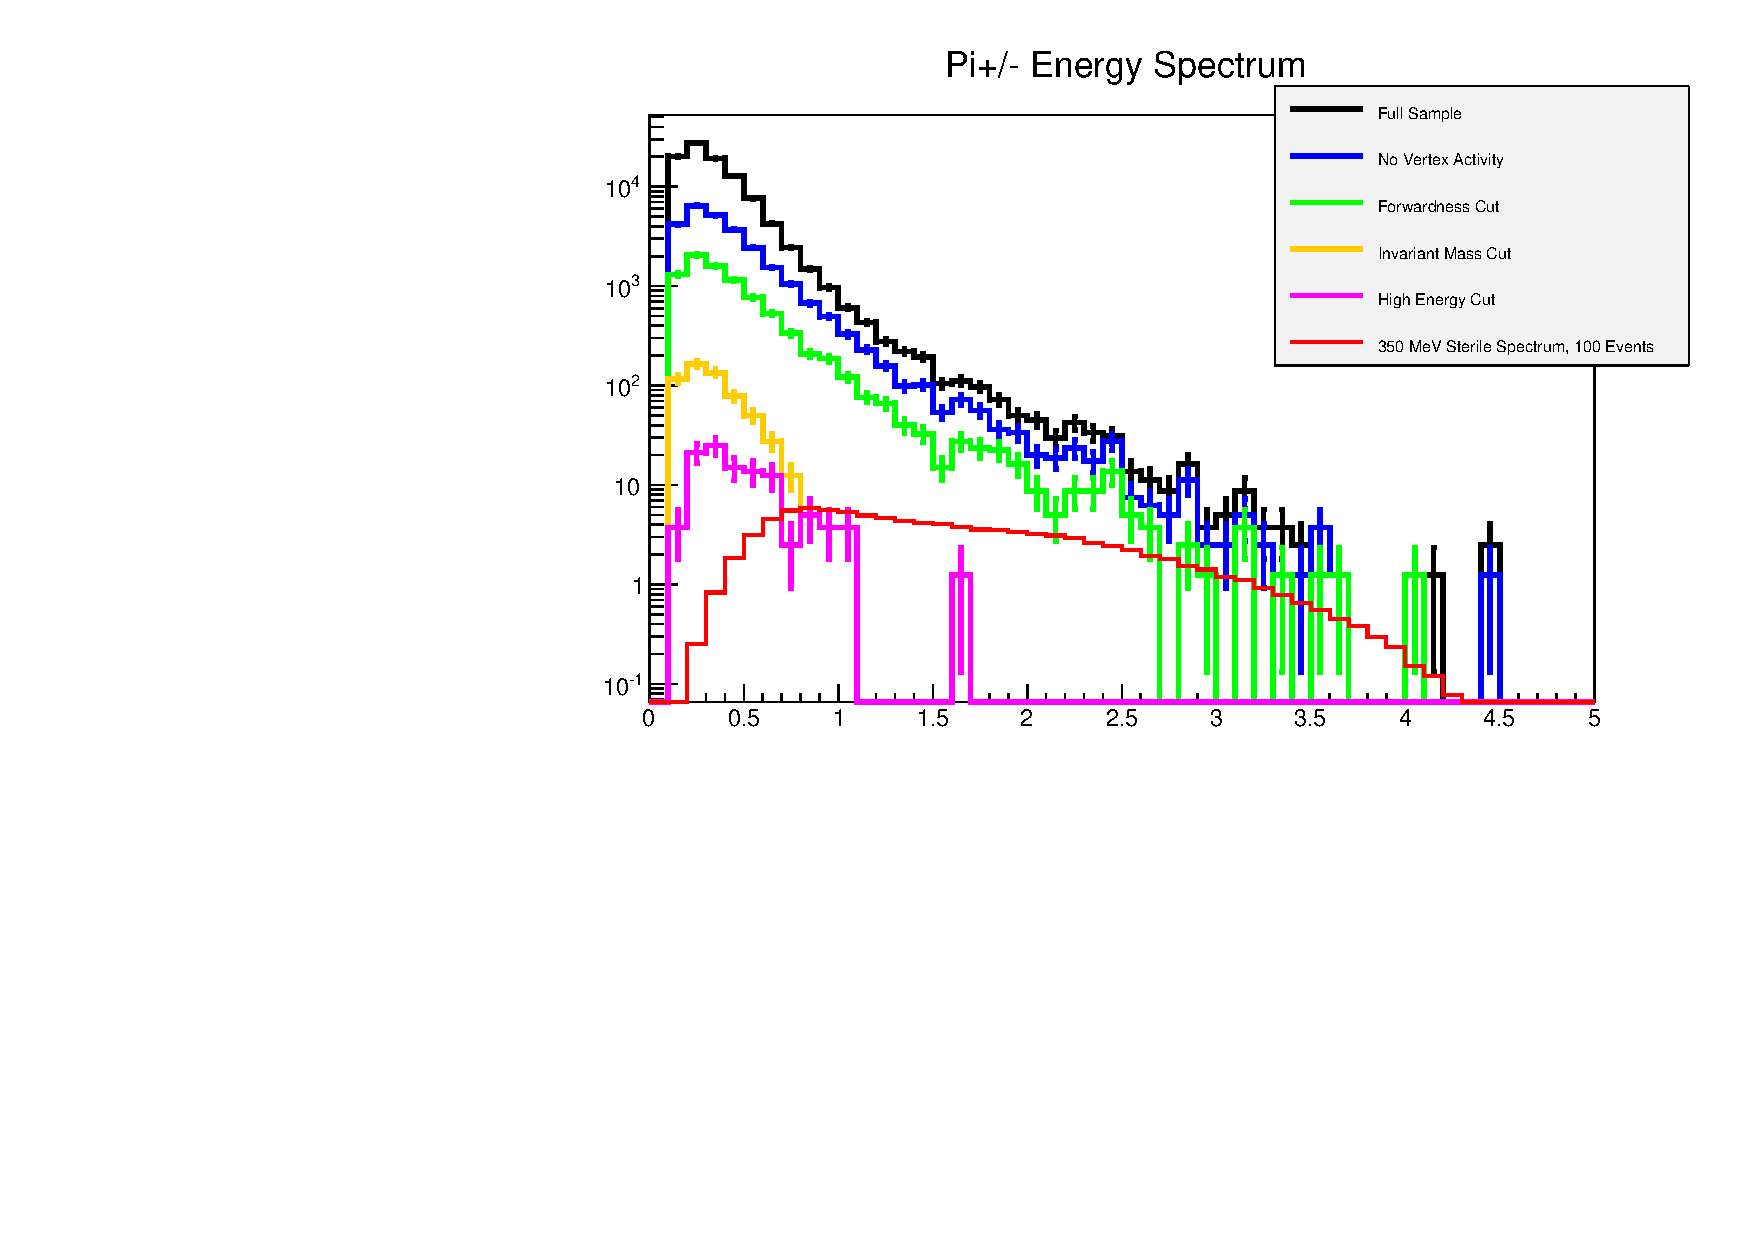
\includegraphics[width=0.7\textwidth]{figures/cuts.pdf}
\caption{\label{fig:cuts} The effect on the background spectra and rate in MicroBooNE to the four main kinetic cuts used to distinguish beam driven scattering events from the decay of a heavy sterile. Also overlayed is the expected signal from the decay of a 350 MeV sterile to $\mu^\pm \pi^\mp$ normalized to 100 events.}
\end{figure}




\begin{table}[t]
\centering
\begin{tabular}{ l | l | l | l}
	Channel & SBND & MicroBooNE & Icarus \\
\hline\hline
\multirow{1}{*}{$\mu^\pm \pi^\mp$} & 1235 & 108 & 176 \\
\multirow{1}{*}{$ e^\pm \pi^\mp$}  & 186  & 17 & 26\\
\multirow{1}{*}{$ \nu \pi^0$}&  -- & -- & --\\
\multirow{1}{*}{$ e^+e^- \text{ (Distinguishable)} $} &  -- & -- & --\\
 \multirow{1}{*}{$ e^+ e^- \text{ (Photon-like)}$} & -- & -- & --\\
 \hline \hline

\end{tabular}
\caption{\label{tab:Rates_post_cuts} A summary of the expected background rates for each channel studied, post cuts. }
\end{table}


\section{Beam Timing}
The above beam related backgrounds are relavent for lower mass steriles, $m_s \leq 50$ MeV and for highly boosted heavy steriles at SBND. Once the sterile becomes less boosted, however, the timing structure of the BNB becomes very relevant for which backgrounds dominate. The Booster neutrino beam consists of 81 Radio-Frequencybuckets of approximately 2ns length, seperated by 19 ns, to form a 19.2$\mu$s spill with a frequency of 3Hz. All events inside this window, alongside all events in the surrounding bins according to assumed resolution, are assumed to be beam-correlated. As can be seen in \ref{fig:timing} below, this is mainly true for light sterile neutrinos at all three SBN detectors, as well as a resonable approximation of heavy neutrino timings at SBND, however, $\mu$BooNE and ICARUS see significant deviation from this with clear peaks in the inter-RF-bucket spacing where one would not expect to see any beam-correlated backgrounds.


\begin{figure}[t]
\center
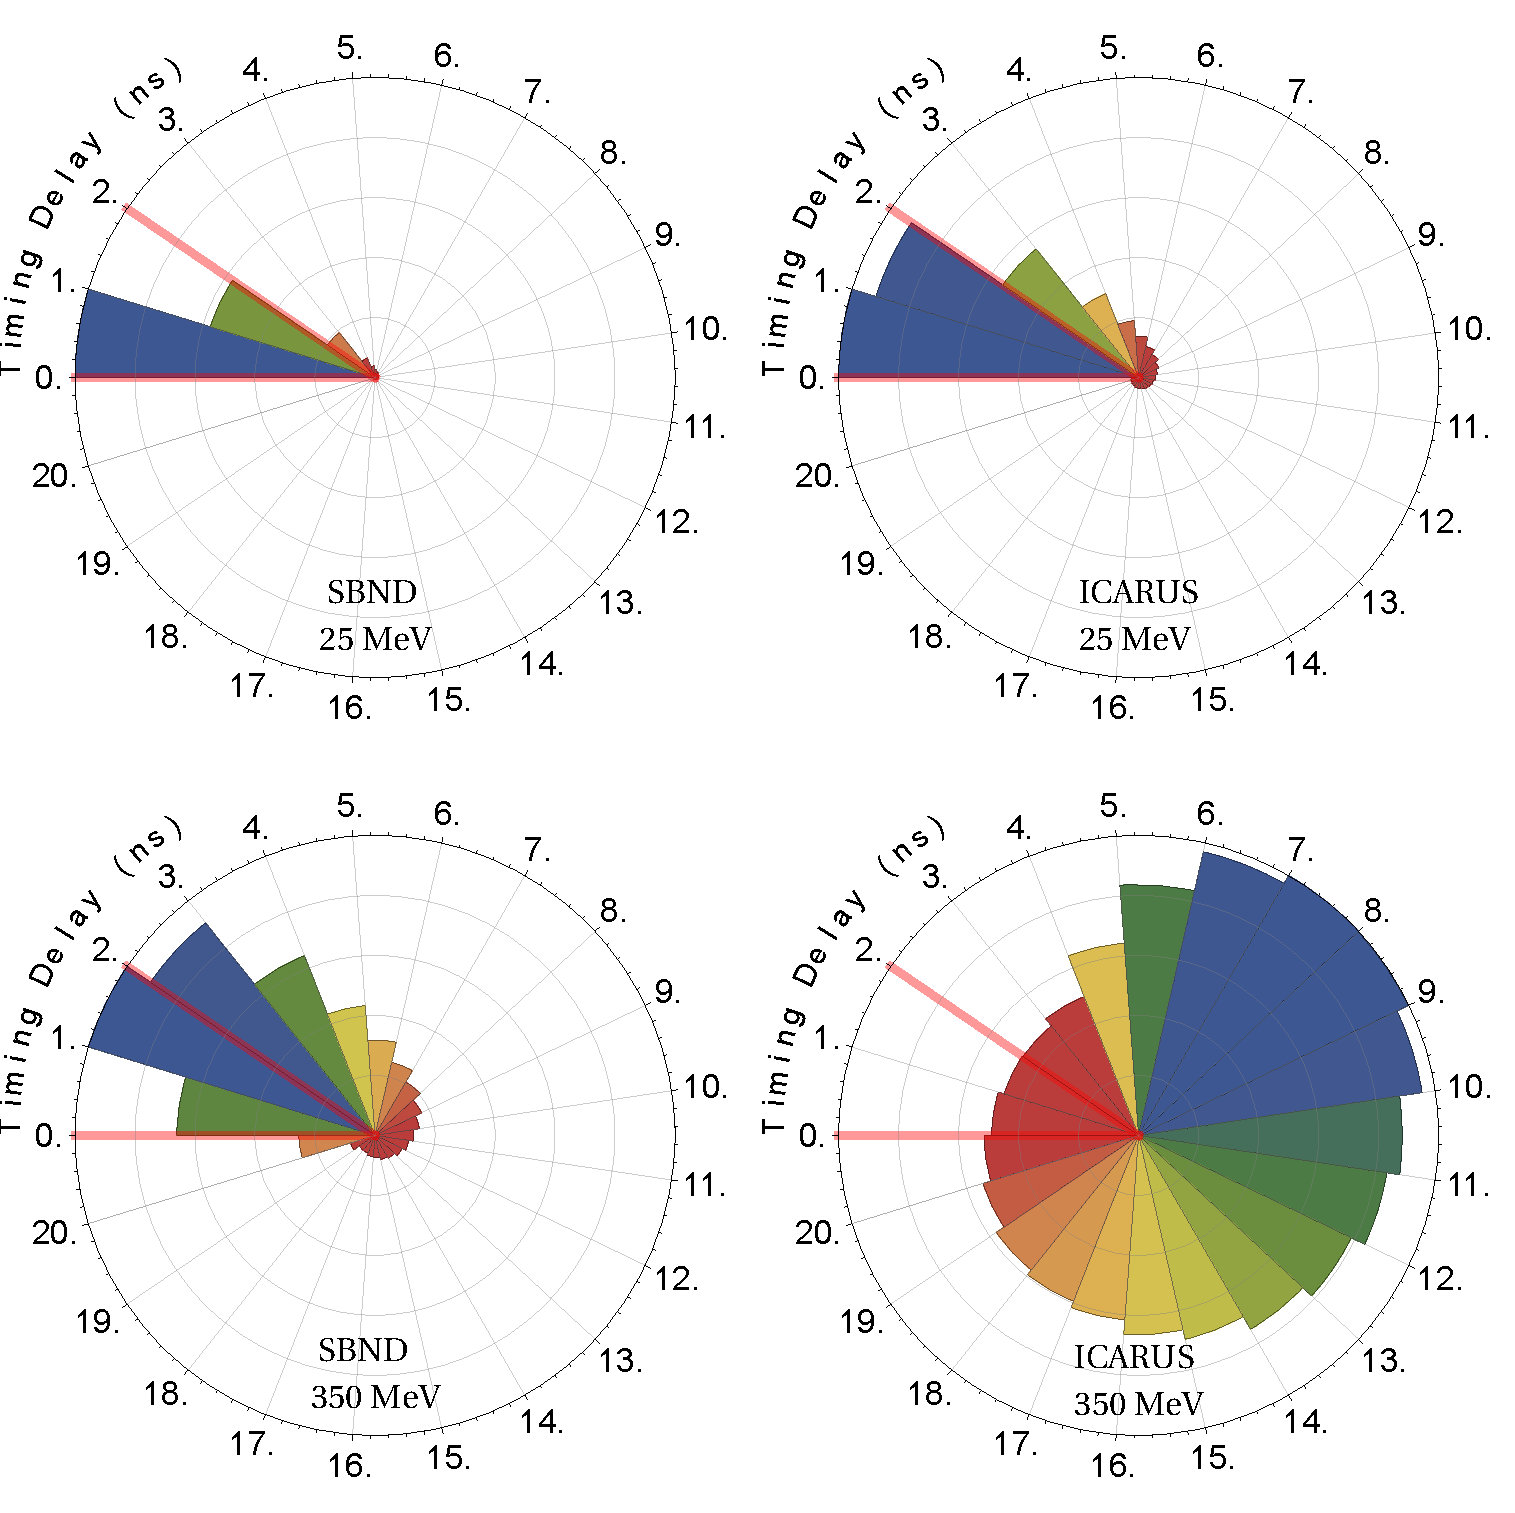
\includegraphics[width=\textwidth]{figures/timing.pdf}
\caption{\label{fig:timing} Shown above is the timing delay of sterile neutrino decays in nano-seconds for both a 25 MeV (top) and 350 MeV (bottom) sterile neutrino at the SBND, $\mu$BooNE and ICARUS detectors (110,470 and 600m respectively). The 2 ns beam bucket window is shown highlighted in red from 0 to 2 ns, followed by an additional 19 ns gap. The timings are calculated as a difference to the time of flight of a active neutrino, assuming the decay occured in a uniform sample accross the 50m BNB decay pipe. A timing resolution of 1 ns is assumed to smear the observed events.}
\end{figure}






\section{Sensitivities}

\subsection{Minimal extension}

In \reffig{fig:no_cuts_no_bkg} we show the sensitivity when cuts are omitted
for backgroundless searches. This corresponds to the most optimistic case:
there are no cuts (weight factors are set to $1$, not even taking into account
physical limitations on the data set) implying perfect signal efficiency, and
the channels are assumed backgroundless.
%
The analysis only considers the total number of events in each channel, and the
contours mark the regions where the detectors in question see more than $2.44$
events, following the procedure of \refref{Feldman:1997qc} designed for
backgroundless searches for rare events. 

To investigate how the presence of backgrounds weaken these sensitivities, we
have performed a rough estimate of the significance of the signal in various
channels. In \reffig{fig:no_cuts_scaled_bkg}, we consider the quantity
$S/\sqrt{\lambda B}$ and plot contours when the parameter is equal to $1$. At
this point, the size of the new signal events from the heavy sterile decays are
equal to the Poisson noise in the experiment under the approximation of no
signal. The parameter $\lambda$ is used to scale the backgrounds, corresponding
to a greater ability to suppresses these events.  We show two regions, the most
conservative line corresponds to $\lambda=1$ with no additional background
suppression beyond our estimates, whilst the more optimistic one corresponds to
a further suppression by a factor of 1000. Our estimates are given by the
largest numbers in \reftab{tab:rates} for each channel, that is assuming no
analysis-based reduction in rates. As before, we do not take into account the
signal efficiency in these plots (weight factors are set to $1$) this makes the
unrealistic assumption that whatever has been done to reduce the backgrounds
leaves the signal event rates unchanged. However, it provides an understanding of 
the severity of the impact of the backgrounds for these searches.

\newtext{PB}{Be careful: the contours aren't really the same thing as the
shaded region, as they are computing different statistical quantities. But to
make them into actual exclusion curves, we would have to minimize over the 2D
space... which maybe we should do... but as we know it takes a bit of work.
Also, the ee flux isn't quite right for a reason I forget at the moment.}


\begin{figure}[t]
\center
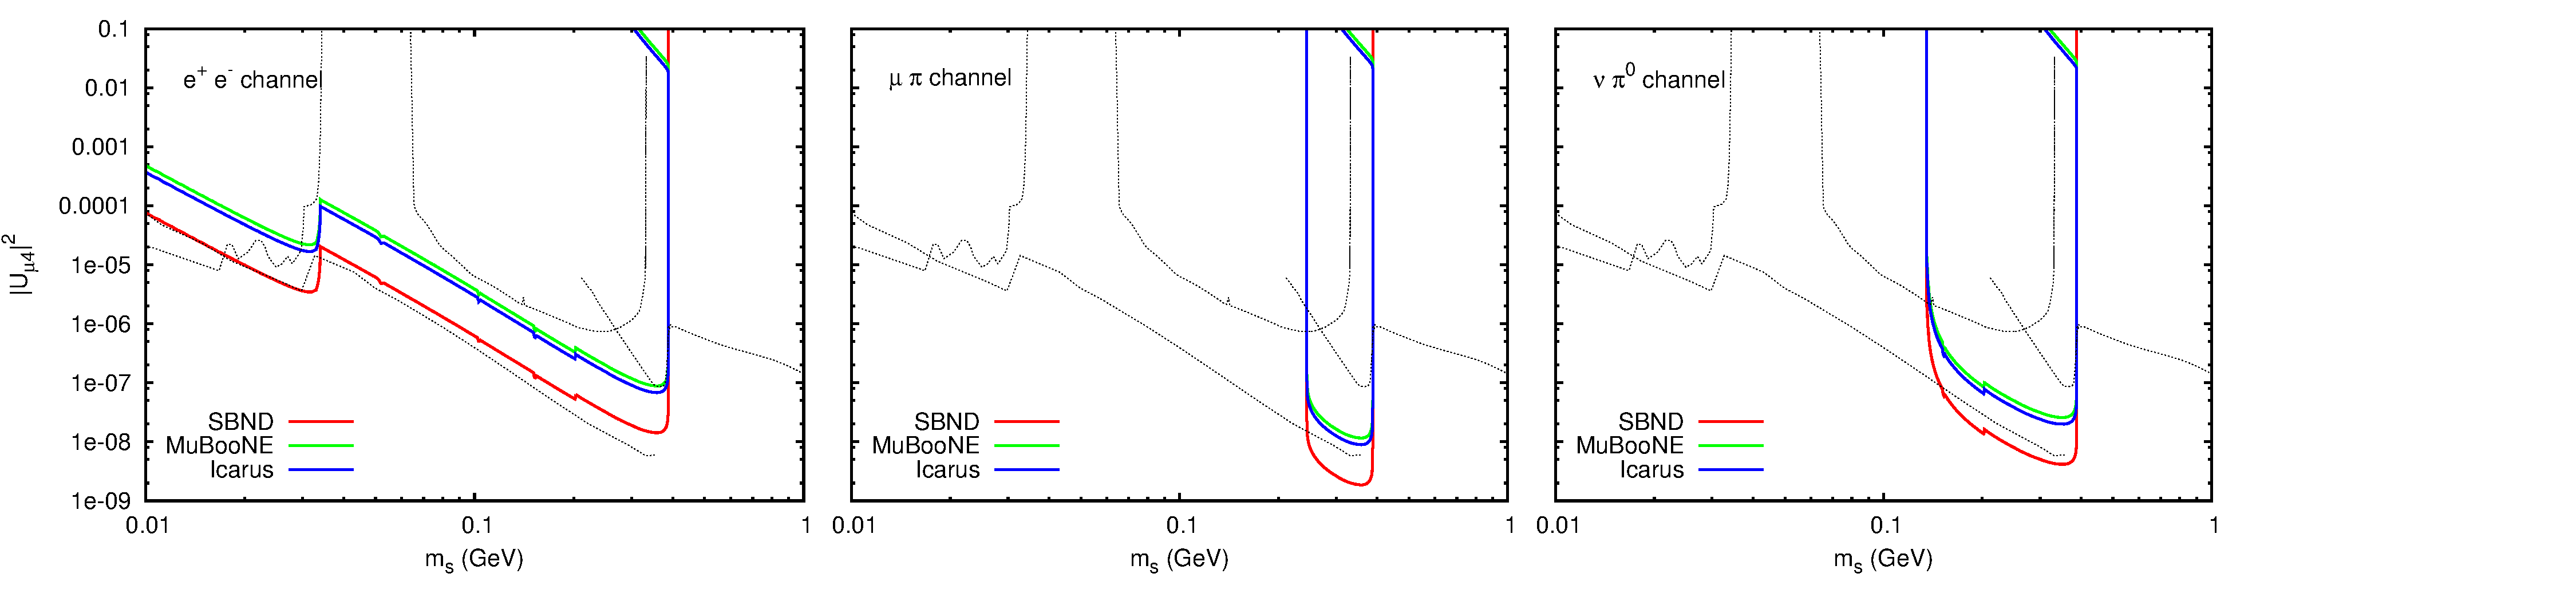
\includegraphics[width=1.0\textwidth,clip,trim=0 20 300 15]{figures/zerobg_um4_all_panels.pdf}
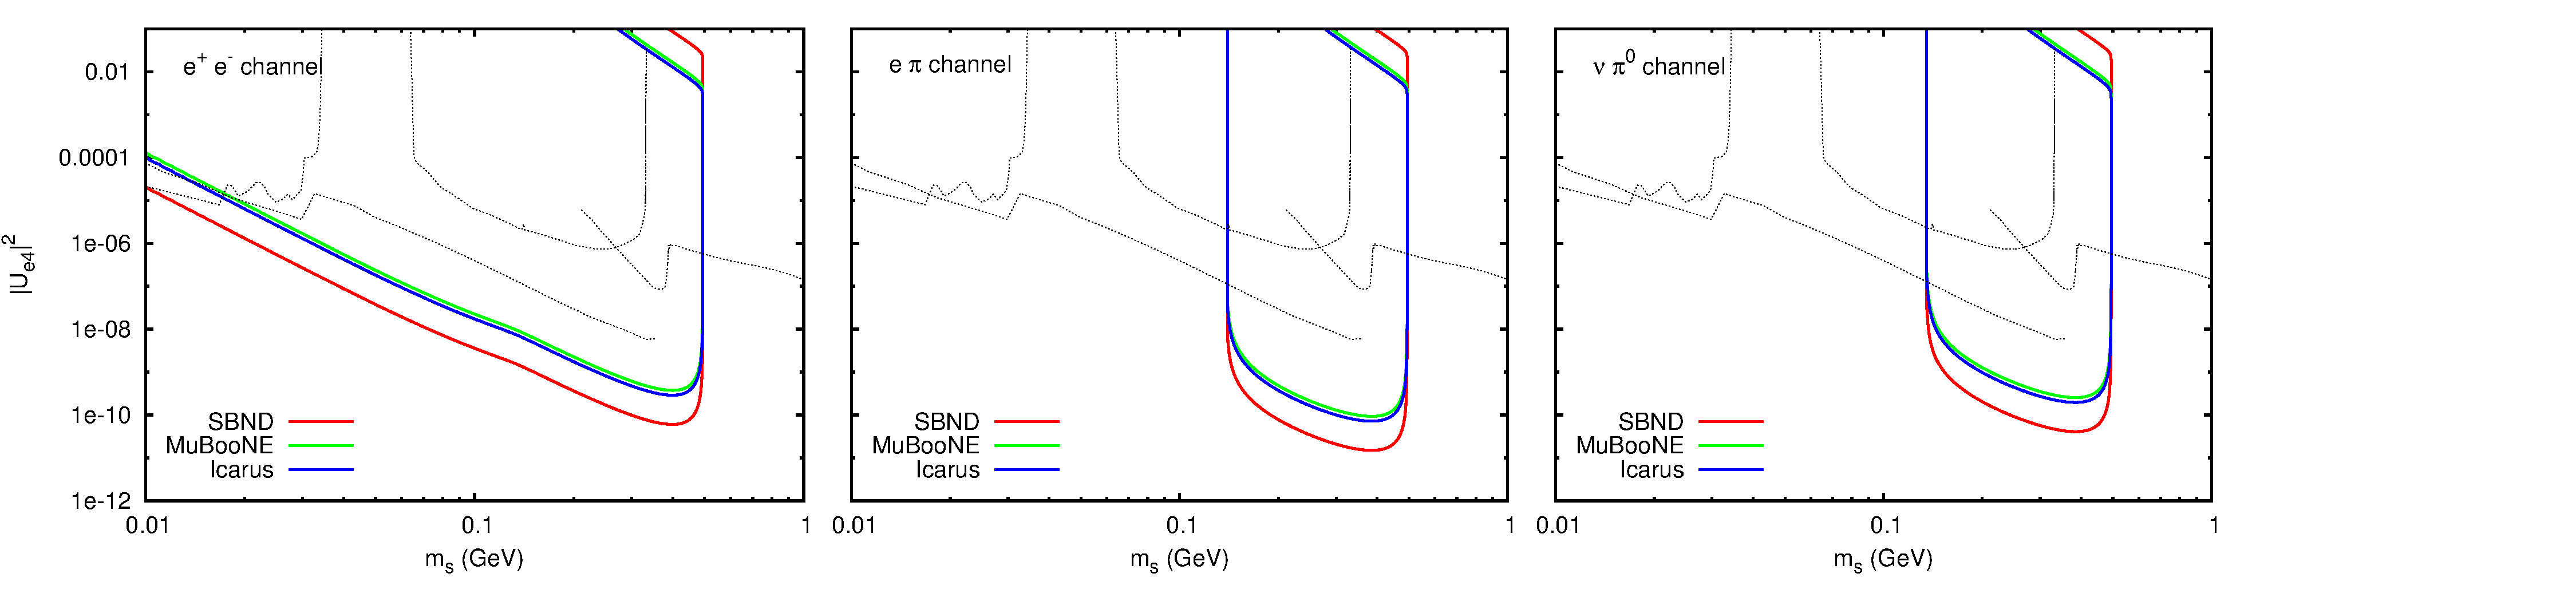
\includegraphics[width=1.0\textwidth,clip,trim=0 20 300 15]{figures/zerobg_ue4_all_panels.pdf}

\caption{\label{fig:no_cuts_no_bkg}The sensitivity contours based on the total number of events, without cuts and without backgrounds. In all panels, the mixing matrix elements not shown on the $y$-axis are zero.}

\end{figure}

\begin{figure}[t]
\center
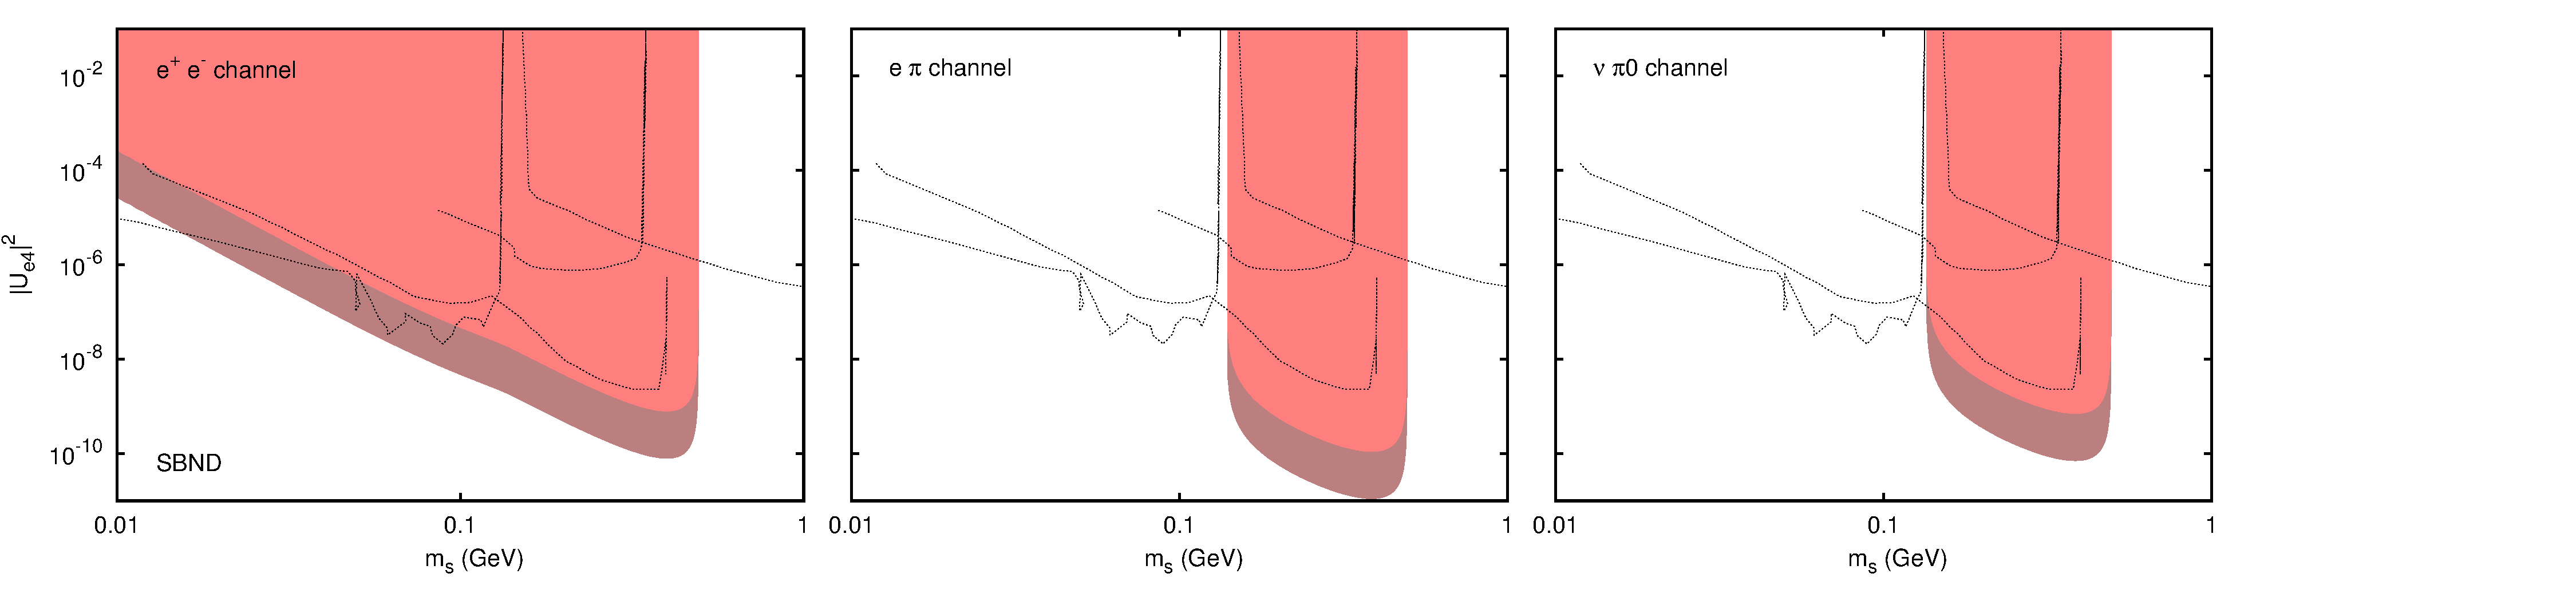
\includegraphics[width=1.0\textwidth,clip,trim=0 20 300 15]{figures/sbnd_all_panels_ue4.pdf}
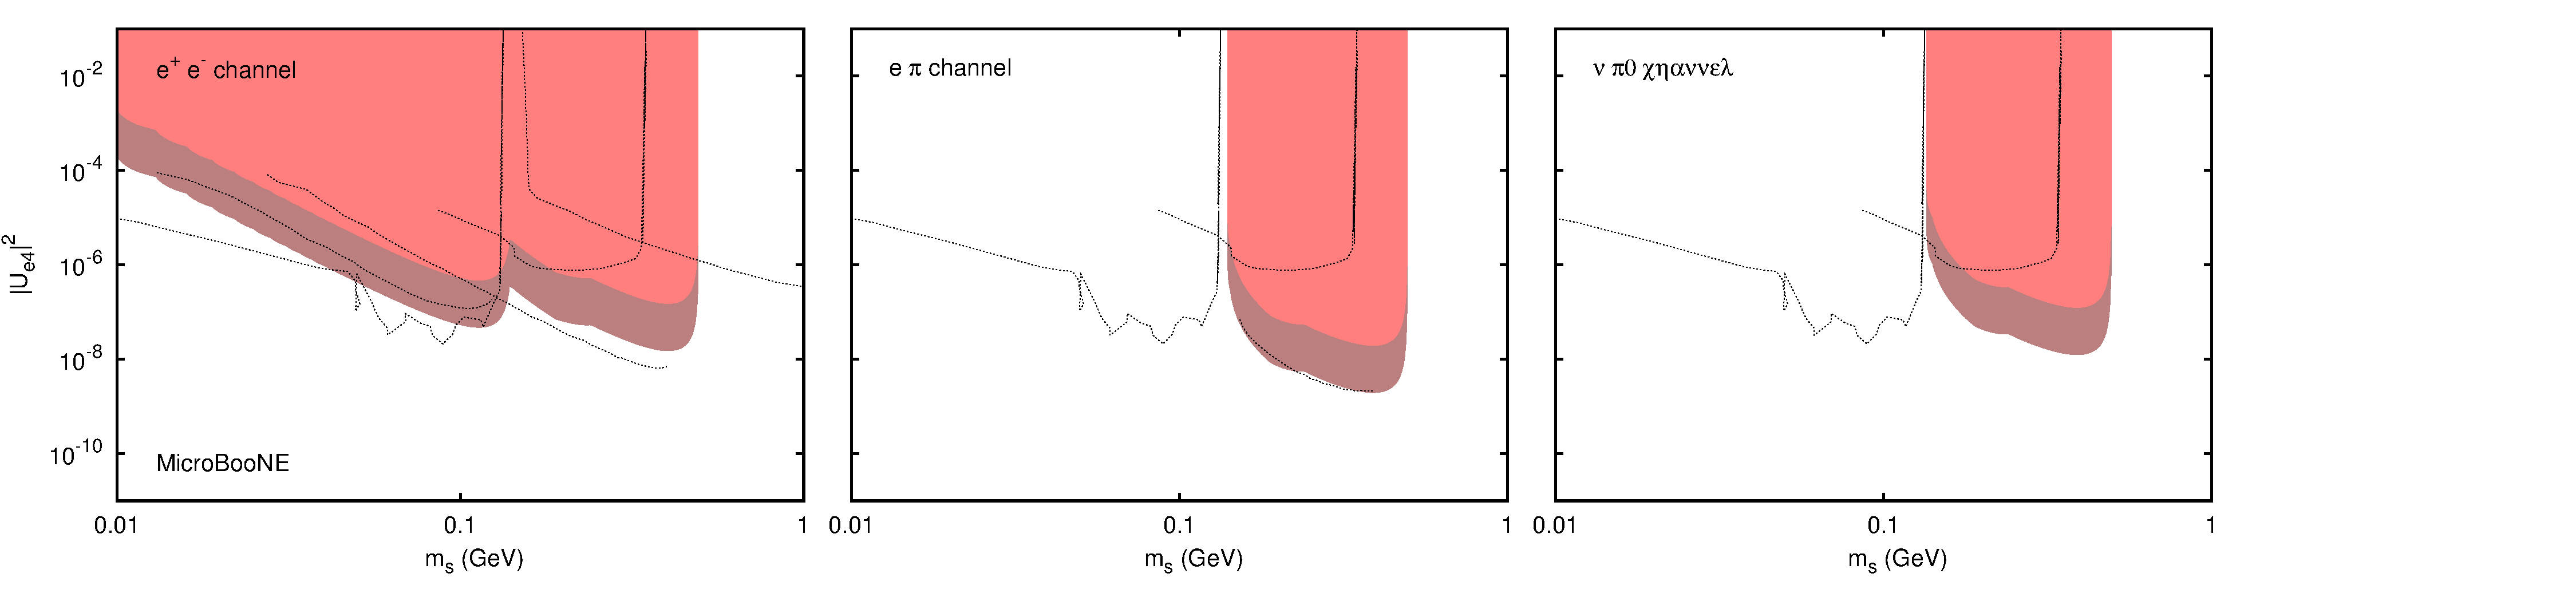
\includegraphics[width=1.0\textwidth,clip,trim=0 20 300 15]{figures/muboone_all_panels_ue4.pdf}
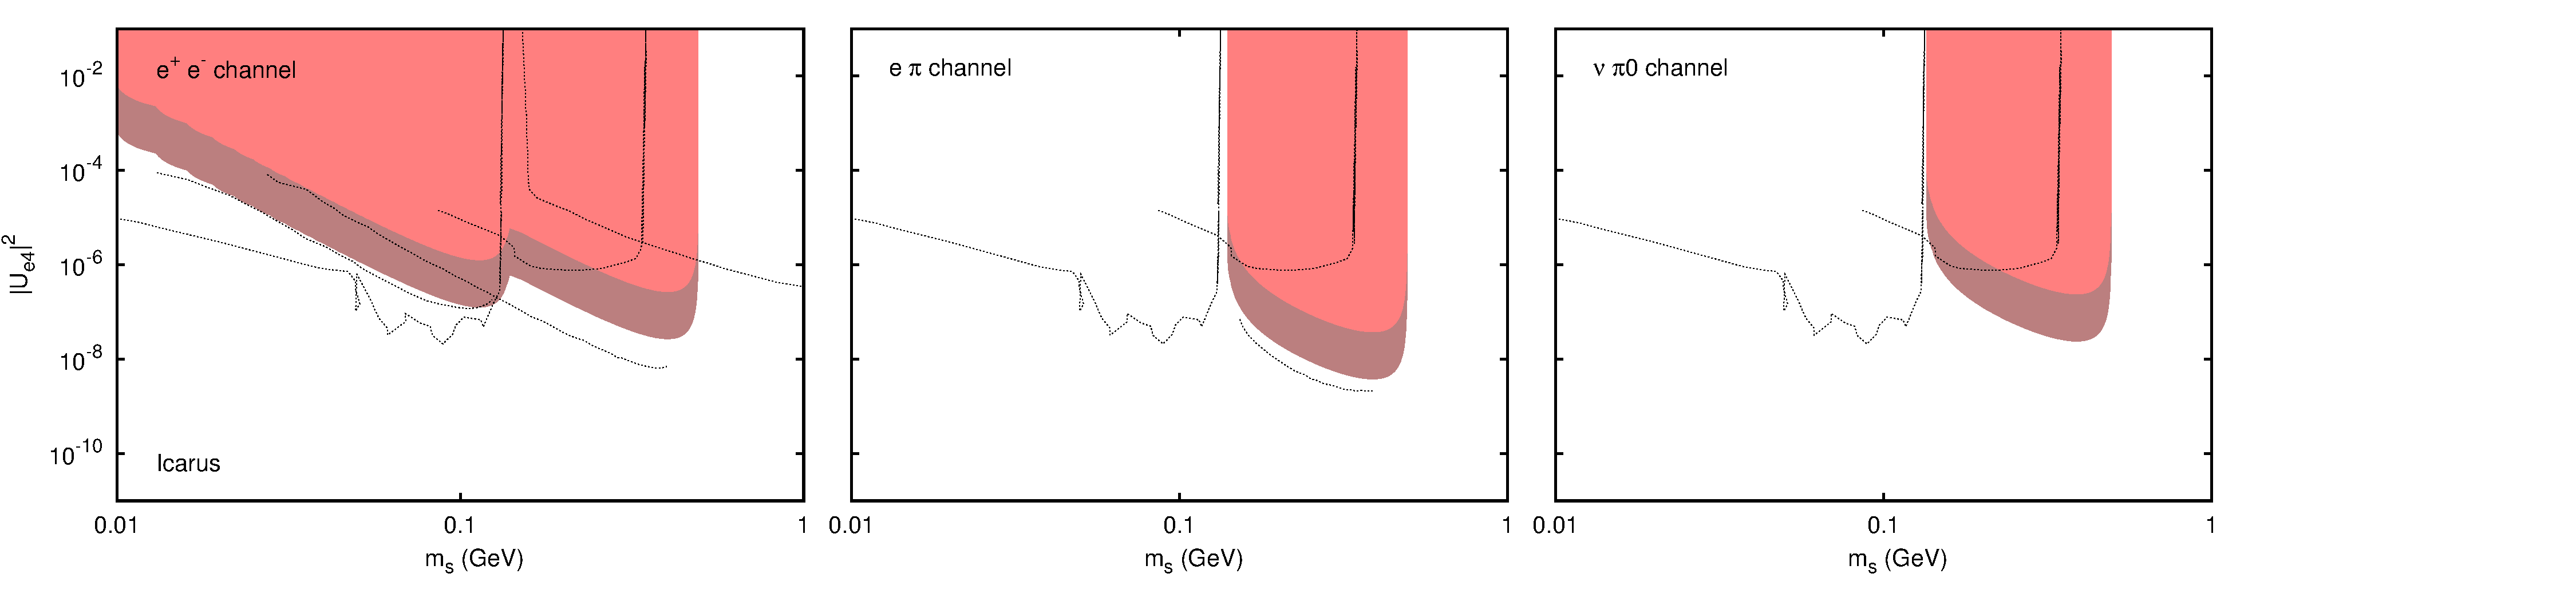
\includegraphics[width=1.0\textwidth,clip,trim=0 20 300 15]{figures/icarus_all_panels_ue4.pdf}

\caption{\label{fig:no_cuts_scaled_bkg_ue4_only}The sensitivity contours based on the total
	number of events, assuming only mixing with the electron neutrino ( $\vert U_{\mu 4}\vert^2=\vert U_{\tau 4}\vert^2=0$), without cuts but with varying degrees of background
suppression. We overlay the 95\% exclusion regions for $U^2$ and $m_s$ from
previous experimental work.}

\end{figure}

\begin{figure}[t]
\center
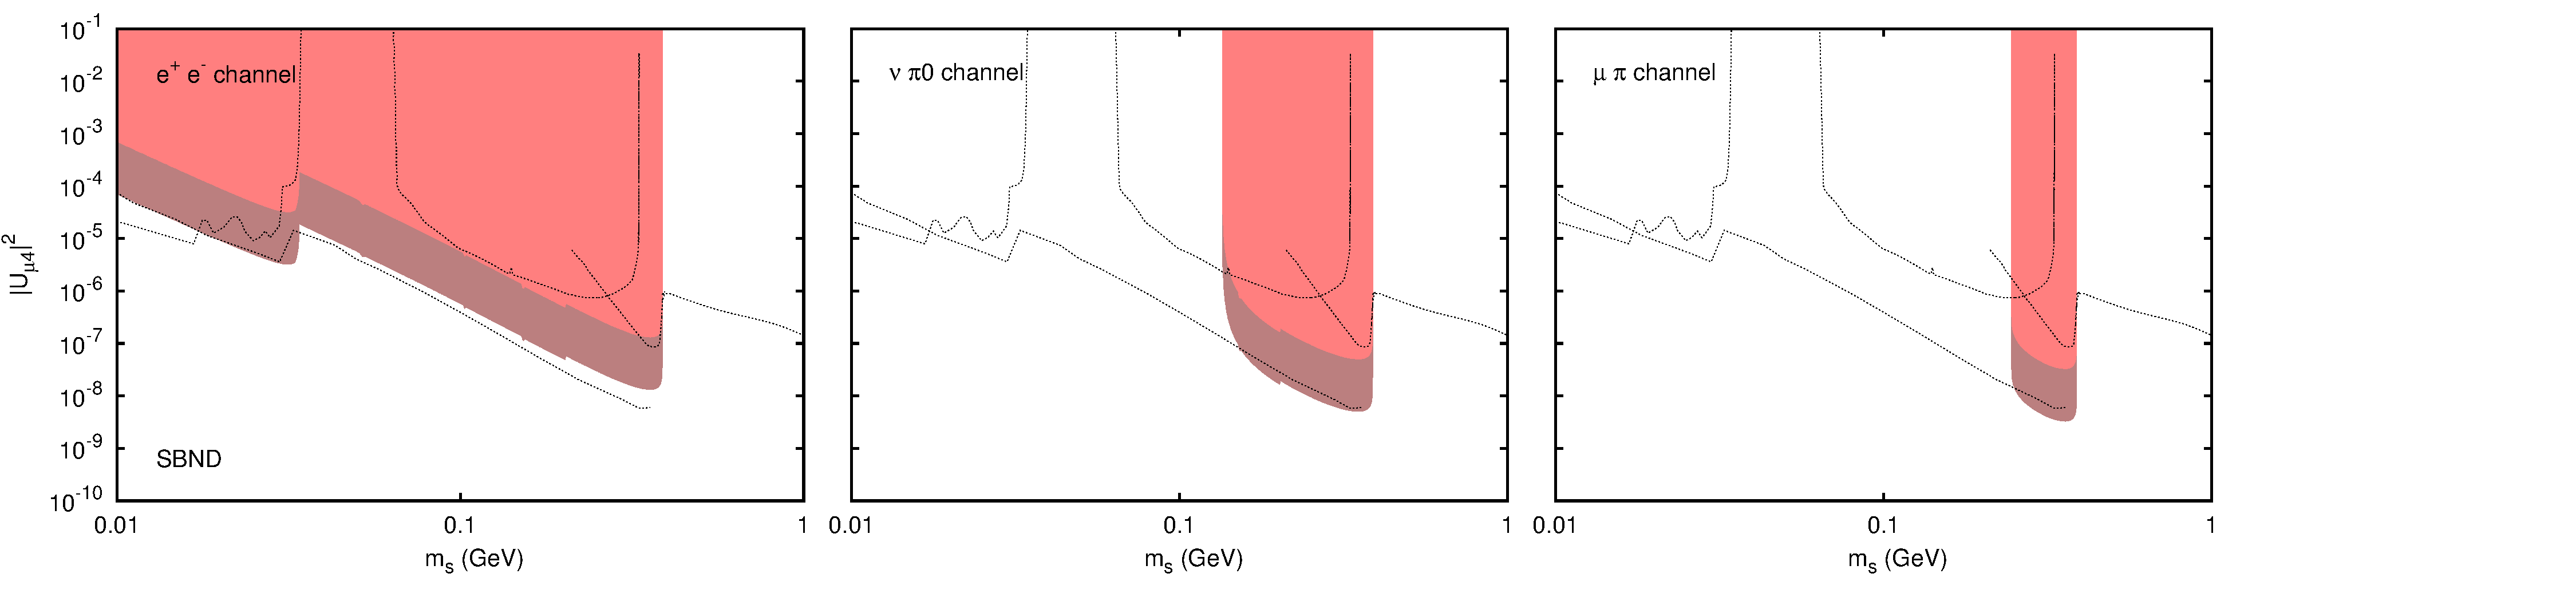
\includegraphics[width=1.0\textwidth,clip,trim=0 20 300 15]{figures/sbnd_all_panels_um4.pdf}
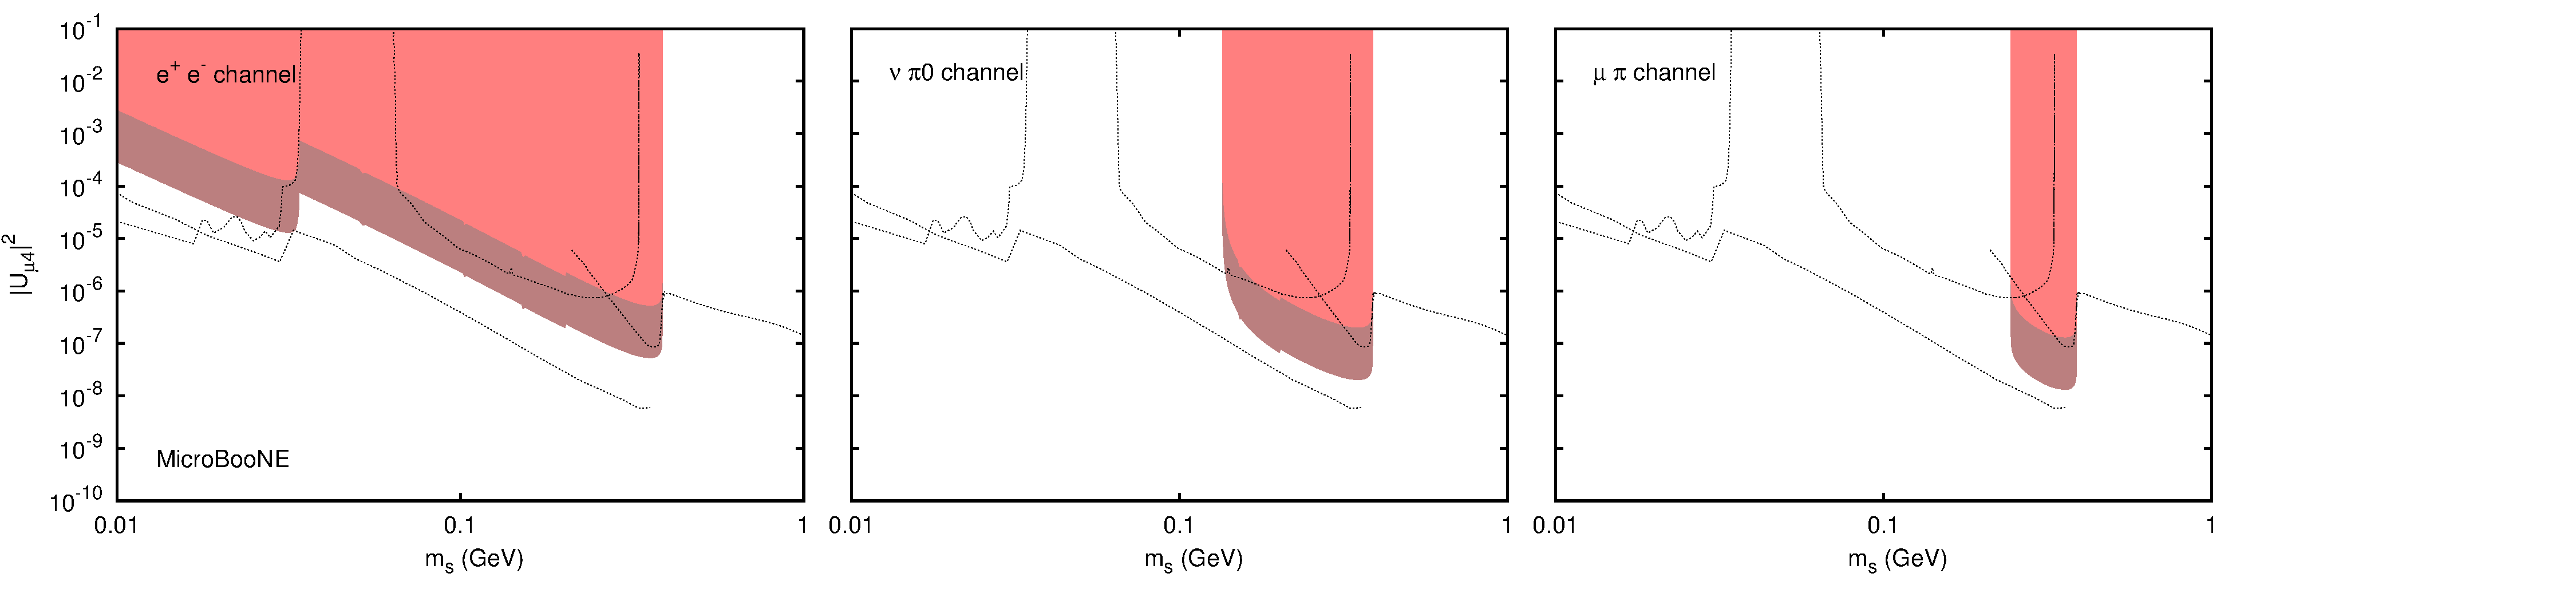
\includegraphics[width=1.0\textwidth,clip,trim=0 20 300 15]{figures/muboone_all_panels_um4.pdf}
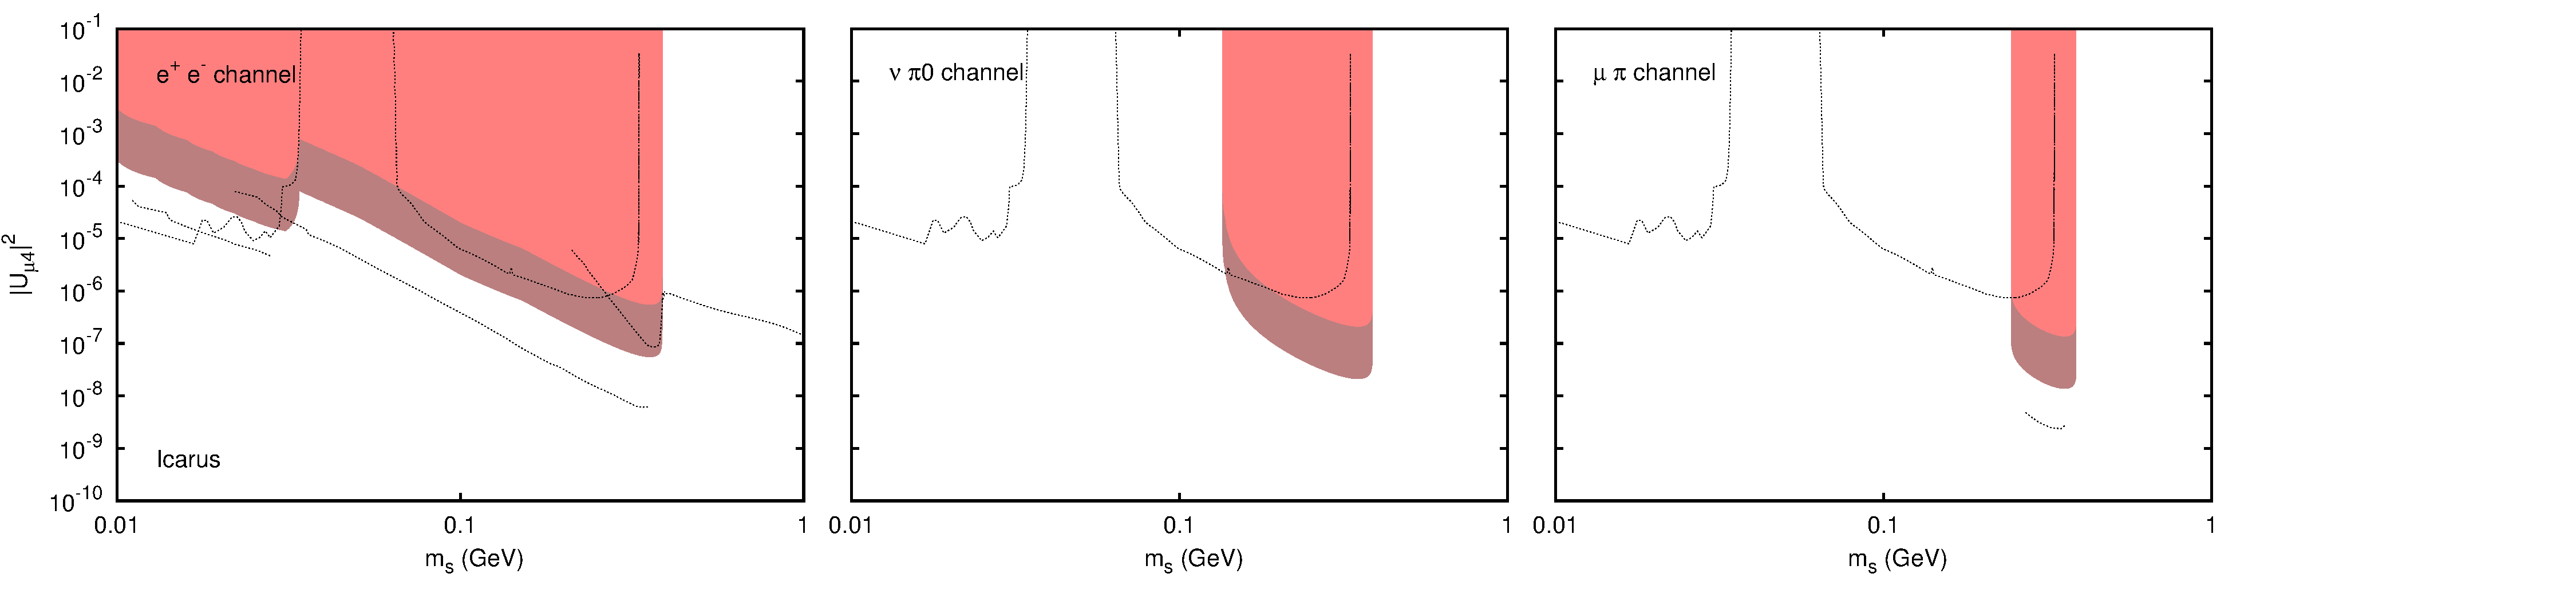
\includegraphics[width=1.0\textwidth,clip,trim=0 20 300 15]{figures/icarus_all_panels_um4.pdf}

\caption{\label{fig:no_cuts_scaled_bkg_um4_only}The sensitivity contours based on the total
number of events, assuming only mixing with the muon neutrino ( $\vert U_{e 4}\vert^2=\vert U_{\tau 4}\vert^2=0$), without cuts but with varying degrees of background
suppression. We overlay the 95\% exclusion regions for $U^2$ and $m_s$ from
previous experimental work.}

\end{figure}



\subsection{Beyond the Minimal Model}

All previous work assumed the minimal extension of one extra sterile degree of
freedom, with no additional physics such that the only decays allowed are
standard model weak processes with an active mixing scaling. 
%
In this model, all interactions of the mostly sterile mass state are produced
by neutrino mass mixing. If the fermion bilinears are removed from the
Lagrangian, the sterile decouples and all (non gravational) observable effects
vanish. An important feature of this model is the all or nothing approach to
decay rates: there is a single parameter, the mixing between the active states
and the mostly-sterile mass state, which dictates the magnitude of all the
decay rates. This is a great asset when trying to constrain the  minimal model,
for example it allows us to place bounds on the observation of $N\to \pi^0 \nu$
despite no experiment to-date reporting the results of such a search. 
%
While this model is minimal in it assumes no new fields or dynamics beyond the
single particle added at observable scales and its renormalizable interactions,
there is no theoretically appealing mechanism to explain a neutral fermion with
a mass below the electroweak scale as well as the sizes of neutrino masses
without the presence of heavier fields in the neutrino sector. The natural
consequence of decoupling these heavy particles would be to generate
non-renormalizable operators which allow for a richer phenomenology for the
intermediate scale sterile than the terms in the minimal extension. Therefore it 
seems relevant to consider models where the minimal interactions produced by 
mass-mixing are supplemented by other operators leading to potentially 
higher decay rates.

In this scenario, the minimal couplings are always present. Therefore, without
suspicious cancellations between the mixing-derived and higher-dimensional
contributions to a decay, the non-observation of a signal in a given decay
channel tells us that the event rate is less than or equal to the bound
produced in the minimal model. The process may still be driven by new physics,
and accordingly we would interpret the factor $U^2$ differently, but the total
rate is bounded in a robust way. However, in the most general extension of the
$\nu$SM we must allow for some decays to be enhanced to a greater extent than
others. This could break the correlation between decay rates present in the
minimal model, and in the case that we are using one channel \emph{e.g.} $N\to
e^+e^-$ to bound another which has not been directly constrained \emph{e.g.}
$N\to\nu\pi^0$, the bounds on the unobserved channel are potentially violated 
and detectable signals could be present.

For the reasons discussed so far, we believe it is relevant to place bounds on
the possible decays of a neutral fermion in an extended scheme which allows for
arbitrary decay rates to visible particles (within the bounds of perturbativity
and other conventional model building constraints).
%
In this section we will consider the possibility of enlarged neutral current
decay rates for the mostly-sterile fermion. In this scenario, the production of
the novel fermion will be largely unaffected by the new physics: heavy states
will be produced in the beam from meson decay via the flavour off-diagonal
charged current interactions as usual. However, we allow for an arbitrary rate
of decay for the three channels
%
\[  \Gamma_{\gamma\nu},\qquad \Gamma_{e^+e^-}\qquad \text{and} \qquad
\Gamma_{\pi^0\nu}. \]
%
 When considering enlarged decay rates, we must be careful with existing bounds
on the model, as an enlarged decay rate would affect all prior beam dump
experiments in the same way until the point where baseline dependence becomes
significant. 


%In order to facilitate the search for new physics we provide results in terms
%of a total scaling $\Gamma$, of each decay channel of interest. We retain the
%functional dependance on sterile mass as in the minimal, bounding $\Gamma \vert
%U_{\alpha 4}\vert^2$. \\

%standard model weak processes with an active mixing scaling. Beyond this there
%are many extensions worth considering, if the sterile sector is charged under a
%new gauge symmetry, e.g $U(1)'$, then the total decay rate can be significantly
%modified. Additional new particle content that couples strongly with the sterile
%states can also drastically change the expected rate with respect to the minimal
%extension, as well as open up entirely new decay channels, such as the possible
%radioactive decay $\nu_N \rightarrow \nu_\alpha \gamma$, which can also be probed
%at the SBN and provides a window to searches for large sterile magnetic
%moments. In order to facilitate the search for new physics we provide results
%in terms of a total scaling $\Gamma$, of each decay channel of interest. We
%retain the functional dependence on sterile mass as in the minimal, bounding
%$\Gamma \vert U_{\alpha 4}\vert^2$. \\

If there was an enhancement of $\alpha$ in a single channel, $\Gamma_c$, such
that the total decay width becomes $\Gamma_\text{tot} =
\Gamma_\text{oth}+\Gamma_c (1+\vert U_{\mu 4}\vert^2 \alpha)$, then previous
experiments searching for heavy sterile decays would have had much more
stringent bounds on $\vert U_{\mu 4} \vert^2$. We can estimate these enhanced
bounds by comparing the probability to decay in a particular channel, with the
probability associated with the published bounds, in particular we need to find
the new value for the 90\% C.L bound, $\vert U_{\mu 4}\vert^2$, such that the
probability to decay inside a detector of baseline L and length $\lambda$, with
a total rate  $\Gamma_\text{tot} = \vert U_{\mu 4}\vert^2
\left(\Gamma_\text{oth}^\prime+\Gamma_c^\prime (1+\alpha)\right)$, is equal to
the probability to decay inside the same detector with total rate
$\tilde{\Gamma}_\text{tot} = \vert U_{\mu 4}^*\vert^2(m_S)
\left(\Gamma_\text{oth}^\prime+\Gamma_c^\prime\right)$, where $\vert U_{\mu
4}^*\vert^2(m_S) $ indicates the published bound on that channel, for a sterile
of mass $m_S$, and primed decay widths indicate the width with mixing removed
to the front. Using the functional form of the probability in equation
\ref{eq:prob}, and expanding to leading order in the assumed small parameter
$\lambda/L$, there are two solutions to this corresponding to the two real
branches of the Lambert-W function. The two solutions correspond physically to
the cases where an increasing decay rate increases the number of observed
events in a detector thus increasing the bound, $\mathcal{W}_0$, up until the
decay rate becomes sufficiently large to ensure the majority of the events
decay before reaching the detector, $\mathcal{W}_{-1}$. This places the 90\%
C.L exclusion in a region \[	-\frac{\vert U_{\mu 4}^* \vert^2}{ \kappa
\Gamma_\text{tot}^{*}} \mathcal{W}_{-1} \left[-\frac{\kappa
\Gamma_\text{tot}^{*}}{1+\alpha} \exp\left(
-\kappa(\Gamma_c^*+\Gamma_\text{oth}^*) \right)     \right]	\geq \vert
U_{\mu 4} \vert^2 \geq \frac{\vert U_{\mu 4}^* \vert^2}{1+\alpha} \] where
$\kappa = \frac{L}{\gamma \beta}$ and we have expanded $\mathcal{W}_0$ to
leading order in $\vert U_{\mu 4}^*\vert^2$ for clarity to see it scales as
expected with enhancement $(1+\alpha)$ , no such convenient expansion exists
for  $\mathcal{W}_{-1}$.  

 
\begin{figure}[t]
%
\centering
%
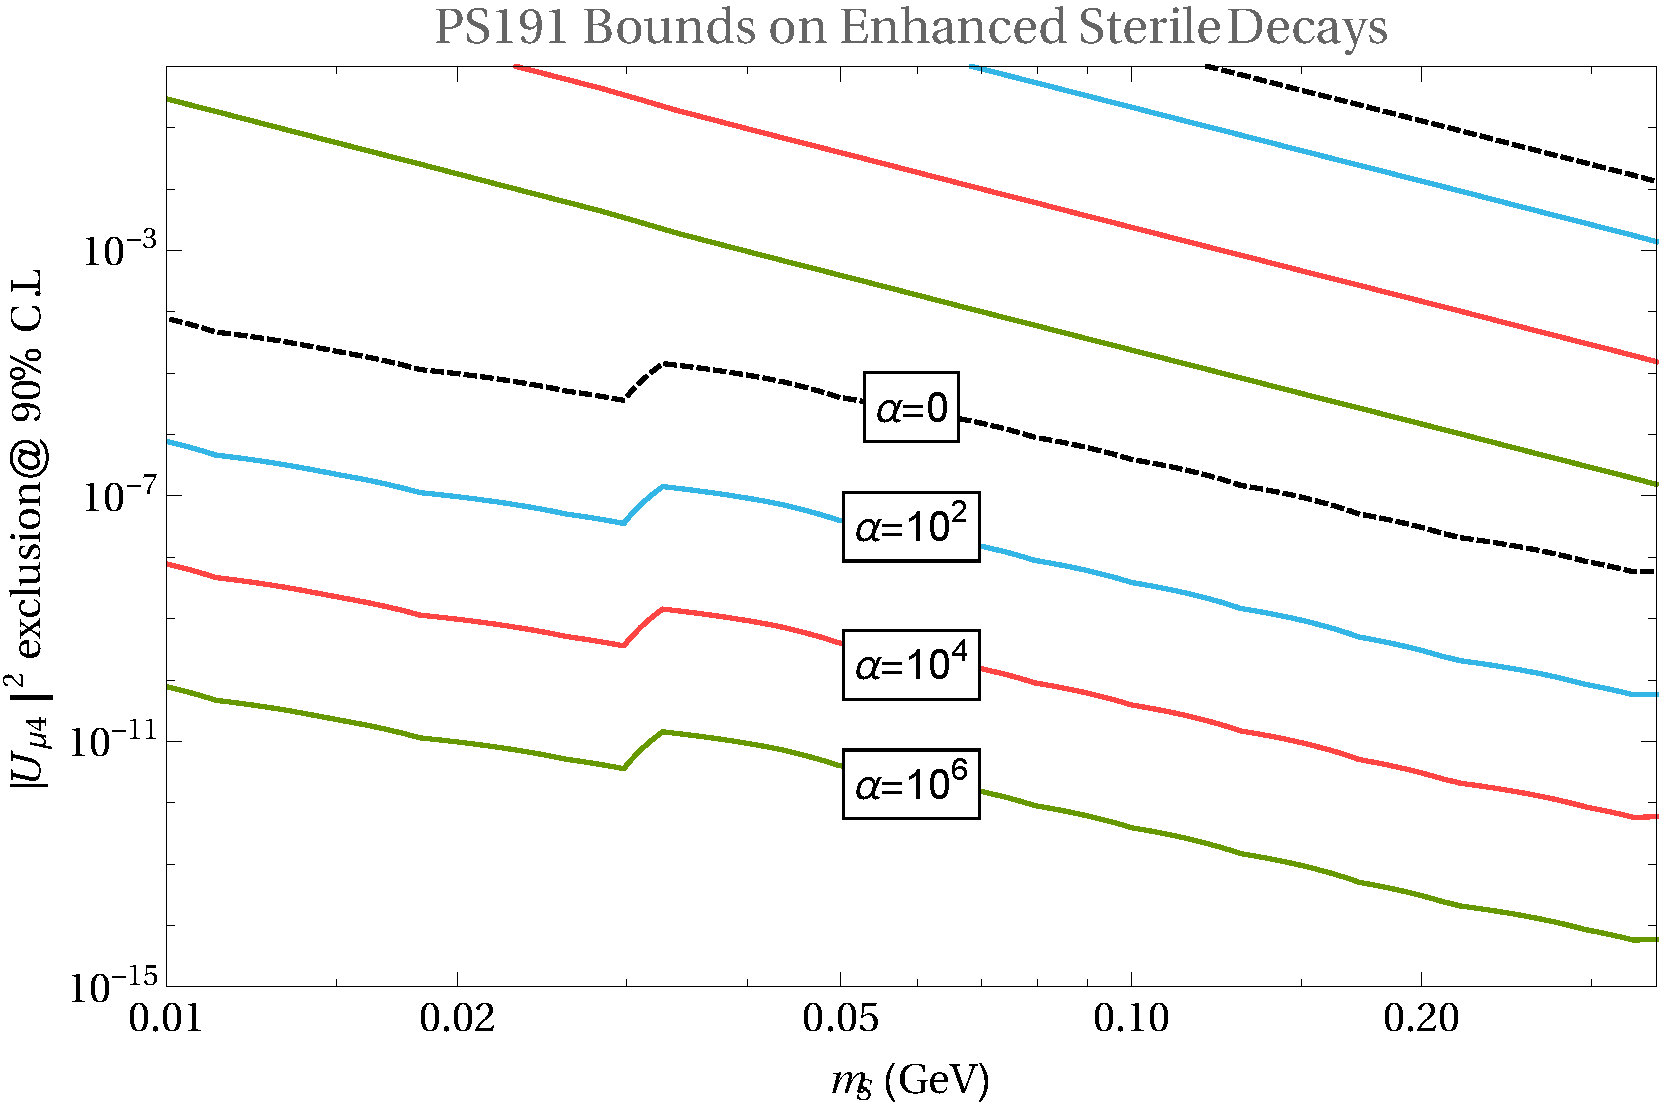
\includegraphics[width=0.49\textwidth]{figures/ps191_enhanced.pdf} 
%
\caption{\label{fig:ps191_enhance}The shifting of bounded region (excluded at
90 \% C.L  between coloured line pairs) as the decay rate to a specific channel
($\nu_N \rightarrow \nu_\mu e^+e^-$) is increased by an arbitrary scaling
factor $\alpha$ at the PS191 facility,$\alpha = 0$ corresponds to the minimal
model bounds. A baseline of 128m, and mean energy of $\left< E_\nu \right>
\approx 1 GeV$ was assumed.  , as well as the }
%
\end{figure}

\section{Baseline dependence at the SBN complex}

The combination of three detectors, all operating with the same technology in
the same neutrino beam allows for distinctive signatures of new physics. By
studying the dependence of the signal on baseline, we could hope to further
constrain the model underlying explanations of any observed excess. 

\begin{figure}[t]
%
\centering
%
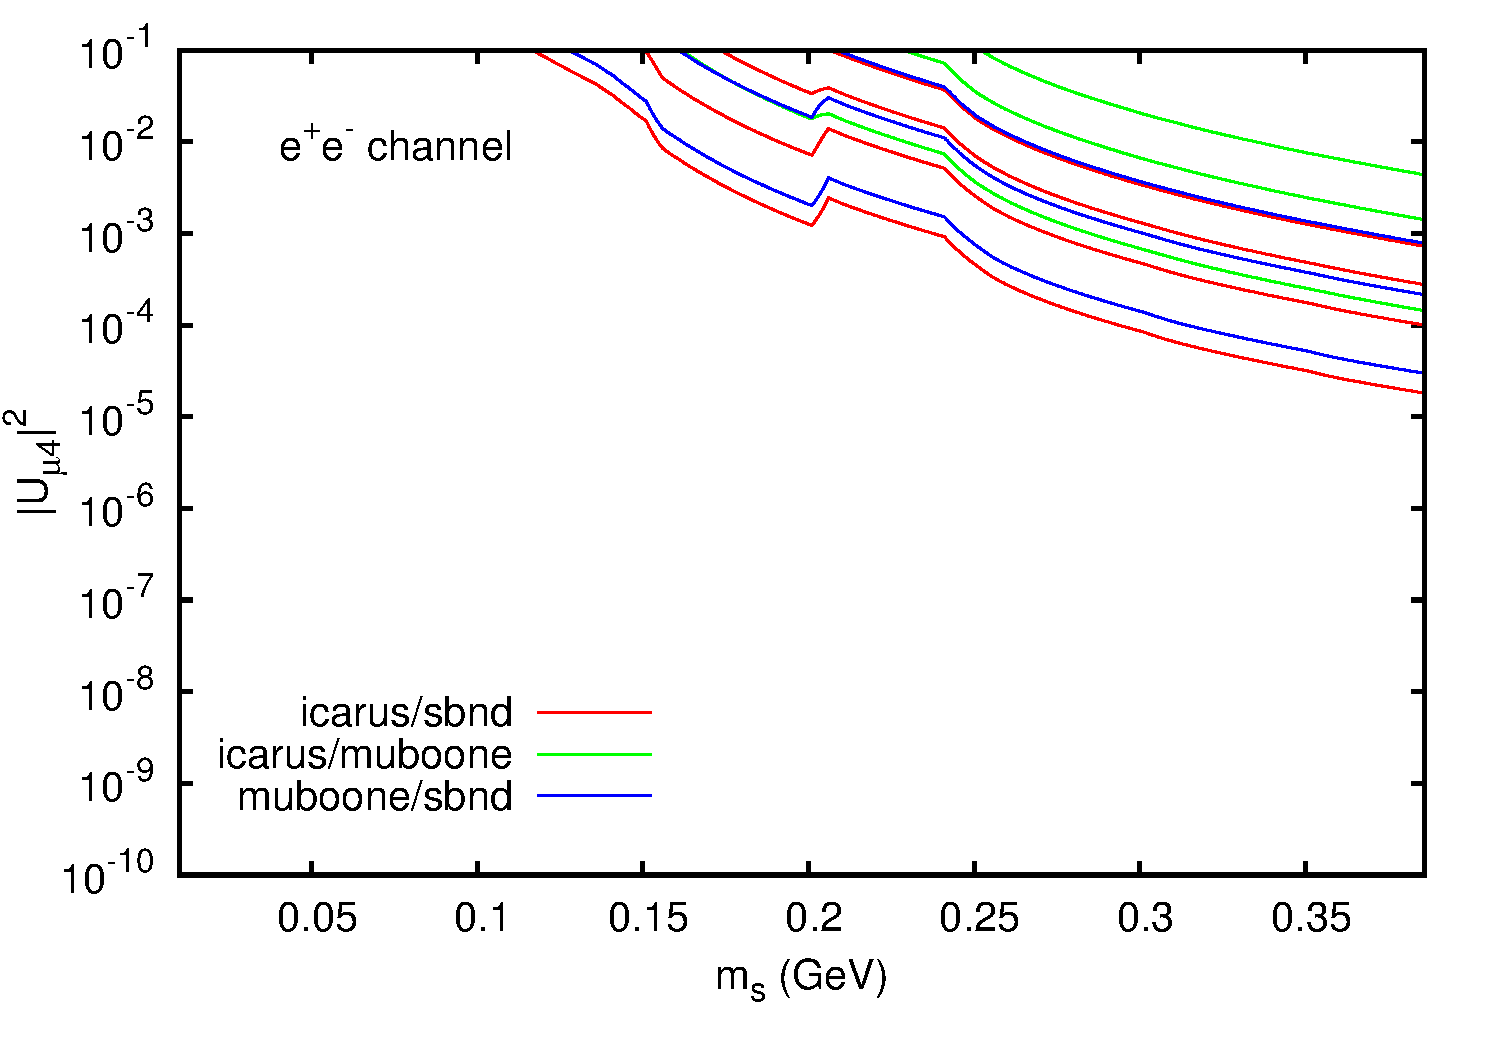
\includegraphics[width=0.49\textwidth,clip,trim=0 20 35 10]{figures/baselineratios_ee_um4.pdf} 
%
\caption{\label{fig:baselineratios} The ratio of event numbers for the $e^+e^-$
decay channel between the three detectors as a function of mass and mixing in
the minimal extension to the SM.  All the regions towards the lower-left
predict a ratio of $1$ between the observed excesses, and the contours show the
lines for excess-ratios of less than 1, 0.75, 0.5 and 0.25. The ratios have been scaled
to account for the dependence of the flux on baseline, and the difference comes
purely from the attenuation of the beam due to decays in transit between source
and detector. }
%
\end{figure}

One of the conventional ways to explain an excess of events at a short baseline
neutrino experiment is through sterile neutrino oscillations. The rates
predicted at three different detectors depend crucially on the respective
distances from source to detector. In the scenarios discussed in this paper, we
also see baseline dependence coming from \refeq{eq:prob}, albeit in a very
different form. For most of the parameter space, we would predict no
significant baseline dependence on the event rates at the three detectors, once
the $1/L^2$ dependence of the flux is removed; however, there for large decay
rates we see a baseline dependent effect. This is shown in
\reffig{fig:baselineratios}, where the event numbers for $e^-e^-$ decay are
shown as ratios between the three detectors. These have been scaled to remove
the baseline dependence of the flux.  The four lines for each detector show the
100\%, 75\%, 50\% and 25\% contours (where the further detector sees fewer
events). Such decay rates are forbidden in the minimal extension of the SM
incorporating MeV scale sterile neutrinos \newtext{PB}{True?}.  

\section{Conclusions}
\lorem\lorem


\newpage 

\section{To do list}

\begin{enumerate}

%\item \sout{Add mass scaling of backgrounds to $S/\sqrt{B}$ plot.}
%\newtext{MARK}{All currently taken care of in centralised file
%"bkg\_event\_rates\_"}

%\item \sout{Work out which mixing angles are active in each plot. And overlay
%$U_{e4}$ bounds on appropriate plot. Probably: recompute plots with this
%information.}

%\item \sout{Plot for total sum of events over detectors.} \newtext{PB}{It's pointless.}

%\item \sout{Add $\nu_e$ flux to \emph{flux.c}.}

\item Actually compute a $95\%$ CL exclusion region for a fair comparison with
bounds. \newtext{PB}{See comment directly below. (This isn't a total
solution... but I spent a while reading about how to do this properly and I
think it's pretty defensible. Perhaps more so than what we would do with
log-likelihood ratios...)}.

\item \sout{The $S/\sqrt{B} =1$ criterion is (if it's defensible at all) really a
$1\sigma$ significance measure. I think we should at least switch it to
$S/\sqrt{B} =2$ which is $2\sigma\approx 95\%$ in the Gaussian limit.}
\newtext{PB}{I have done this and updated the plotting scripts.}

\item Recompute sensitivities for reasonable cuts? Vary the backgrounds
according the cuts and Mark's estimates?

%\item \newtext{PB}{I have added the $(1+\alpha)$ scaling functionality. I only
%ran one test... but it seems to work. I'll try to test more tomorrow.} 

%\item \sout{Play about with baseline distance? \newtext{MARK}{What can we
%really say here, if we limit to "standard" mixing picture  then there isnt a
%huge ammount of results, (see figures/baseline\_effects.pdf), might look into
%increased decay rates?} \newtext{PB}{Yes, I'm starting to think that we should
%just add a section looking at generic decay widths in specific channels... we
%have to make some decisions about how $\Gamma$ scales with $U$. I mean, just
%assuming the minimal extension \emph{is} pretty conservative for theorists.}}
%\newtext{PB}{I think we agreed to just do this.}

\item Turn on $U_{\tau 4}$,$U_{\mu 4}$ and $U_{e4}$ simultaneously. Also look
at ratios of channels and ratios of events to see if we can get any (broken)
degeneracies that could actually be interesting \emph{i.e} SNO style
complementary measurements.

%\item \sout{Edit how the code deals with cuts and efficiency files.
%``--no-cuts" shouldn't need a dummy file of 1's. Maybe a flag ``--cuts-XXX``
%where XXX is either a file name, or ``none'' for which all is handled
%internally.} \newtext{PB}{Now there is a ``--cuts'' flag. ``--cuts=none'' or
%``-cuts none'' sets all weights to 1 internally. Or you can pass it a file name
%``--cuts=eff.dat'', which works as expected. Default is no cuts, but I've
%updated the scripts to have the right flags.}

%\item \sout{Write code for general $\Gamma$ for different final state
%particles.} \newtext{PB}{I've had a first pass at this. I didn't write new
%decay channels in the end, as I think we can just rescale things...  depending
%on how we choose to scale the $\Gamma$ with $U$ and $m$ (see below), we could
%change this later, but for now it seemed OK. Now there's a new command
%line argument which adds an extra Gamma to whichever channel you specify as well 
%as the total decay rate \emph{e.g.} \texttt{eventrate --mupi --extra-gamma 1e-18}
%adds a constant $1\times10^{-18}$ to the $\mu\pi$ channel and total rate (not
%double counting). When we write a function like \texttt{loop\_muon\_enhanced\_gamma()} we 
%can set this extra gamma to depend on $U$ or $m$ as we need.} 

\item Write a section talking about the motivation for non-minimal extensions,
specifically enhanced $\Gamma$. Discuss the breaking of the relationship
between $\Gamma$, $U^2$ and $m_s$.  Make a reasonable suggestion for possible
scaling behaviours of $\Gamma$ on $U^2$/$m_s$. Is it as boring as rewriting the
minimal decay rate with $G_F$ replaced by a new constant that isn't suppressed
by the $W$-mass? Or can you get different scaling behaviours from new physics? \newtext{PB}{Let me know if you want to look at this today: 16 Feb.}

\item Based on the point above: decide how we can make plots for this. How do
we compute the bounds? I guess, the bounds are \emph{really} bounds on
$U^2\Gamma$? What's the best way to display the three dimensional data etc.
Make the data. Make the plots.

\item \sout{Cosmogenics? Ignorable? Write up if/so/why/how?} More depth needed.

\item \sout{Can prob be used to fudge a bound scaling? i.e for PS191.}
\newtext{MARK}{In the end I felt it easiest to just add PS191 as a new detector
in the code. This was it is easy to call for probability shifts, and gives us a
CHECK if we can reproduce the known bounds somewhat.  --using-ps191 with the
CHAN\_FLAG of 4.  This "Detector" has correct POT, dimensions, baseline ..etc..
although the associated flux is assuming the BNB beam (which is wrong, but
probably not insanely wrong). I also wrote two new functions to call the upper
and lower 90\% C.L bounds from an experiment, given the observed bound.
Although currently bounds are done out of code in the plotting scripts, needs
to be updated then. }

\item \newtext{PB}{I have added the $(1+\alpha)$ scaling functionality. I only
ran one test... but it seems to work. I'll try to test more tomorrow.} 

\item \sout{PS191 replicate the bounds.} \newtext{MARK}{Consistently a factor of $\approx 100$ off. What Ive checked. Fluxes seem good. We are using same $\Gamma_{\nu ee}$, up to I integral. POT is good. L, and $\lambda$ as well as other dimensions seem good. Hmm. Effect is really only in $\vert U_{\mu 4}\vert^2$ and not electron, checking meson-BR. Not meson-Br. FIXED! although still $\approx 50$ off. Lets say conservative.} 
	We are still missing that factor of 50. Total decay rate is irrelavent, only channel is important. is channel correct?

\item Generating the electron and electron-like signal, as well as simpley more stats \newtext{MARK}{working on this}

\item Interesting ways to compare baseline for different signals and backgrounds. See figure \ref{fig:baseline_comp} below.





\item Just a small note to (maybe?) clarify the situation involving the two body decay kinematics. I noticed that when the particle is massless I couldnt not get any sort of maximum or minimum in the lab frame angle. However, I wasn't sure that the two effects are exactly related (the rounded curve and the spikes to 0 angle) so I looked at the massive daughter case. So looking at $\pi^+ \rightarrow a+b$, with $m_a$ small but non-zero, and stared componants in the rest-frame of the pion.
	\begin{align}
		P_a &= (E_a, |p_a| \sin \theta, 0, |p_a| \cos\theta ) \\
		    &=(\gamma E_a^*+ \beta_\pi \gamma |p_a^*| \cos \theta^*, -,-,\gamma \beta_\pi E_a^* + \gamma |p_a^*| \cos \theta^*)
	\end{align}
	so we can construct the lab frame angle, with $\beta_a = |p_a^*|/E_a^* \approx 1 - \epsilon$, 
	\begin{align}
		\cos \theta &= \frac{\beta_\pi+\beta_a \cos \theta^*}{1+\beta_\pi \beta_a \cos \theta^*} \\
							       &= \frac{c^*+\beta_\pi}{1+c^* \beta_\pi}+\epsilon \frac{c^*(-1+\beta_\pi^2)}{(1+c^* \beta_\pi)^2} + \mathcal{O}(\epsilon^2)
	\end{align}
	Varying the the rest frame angle we see the maximum and minumum angles in the lab frame are given by $\theta^* = -1$ and $1$ 
	\begin{align}
		\cos \theta^{\text(max,min)} &=  \frac{\beta_\pi \pm \beta_a }{1 \pm \beta_\pi \beta_a} \\
	\end{align}
	Please see figure \ref{fig:boost} for the basic results. This gives a pretty good reason as to why there is a minimum angle. However, it does not help with the arms and angles when there is a large massive particle. 

	\end{enumerate}

\begin{figure}[t]
\center
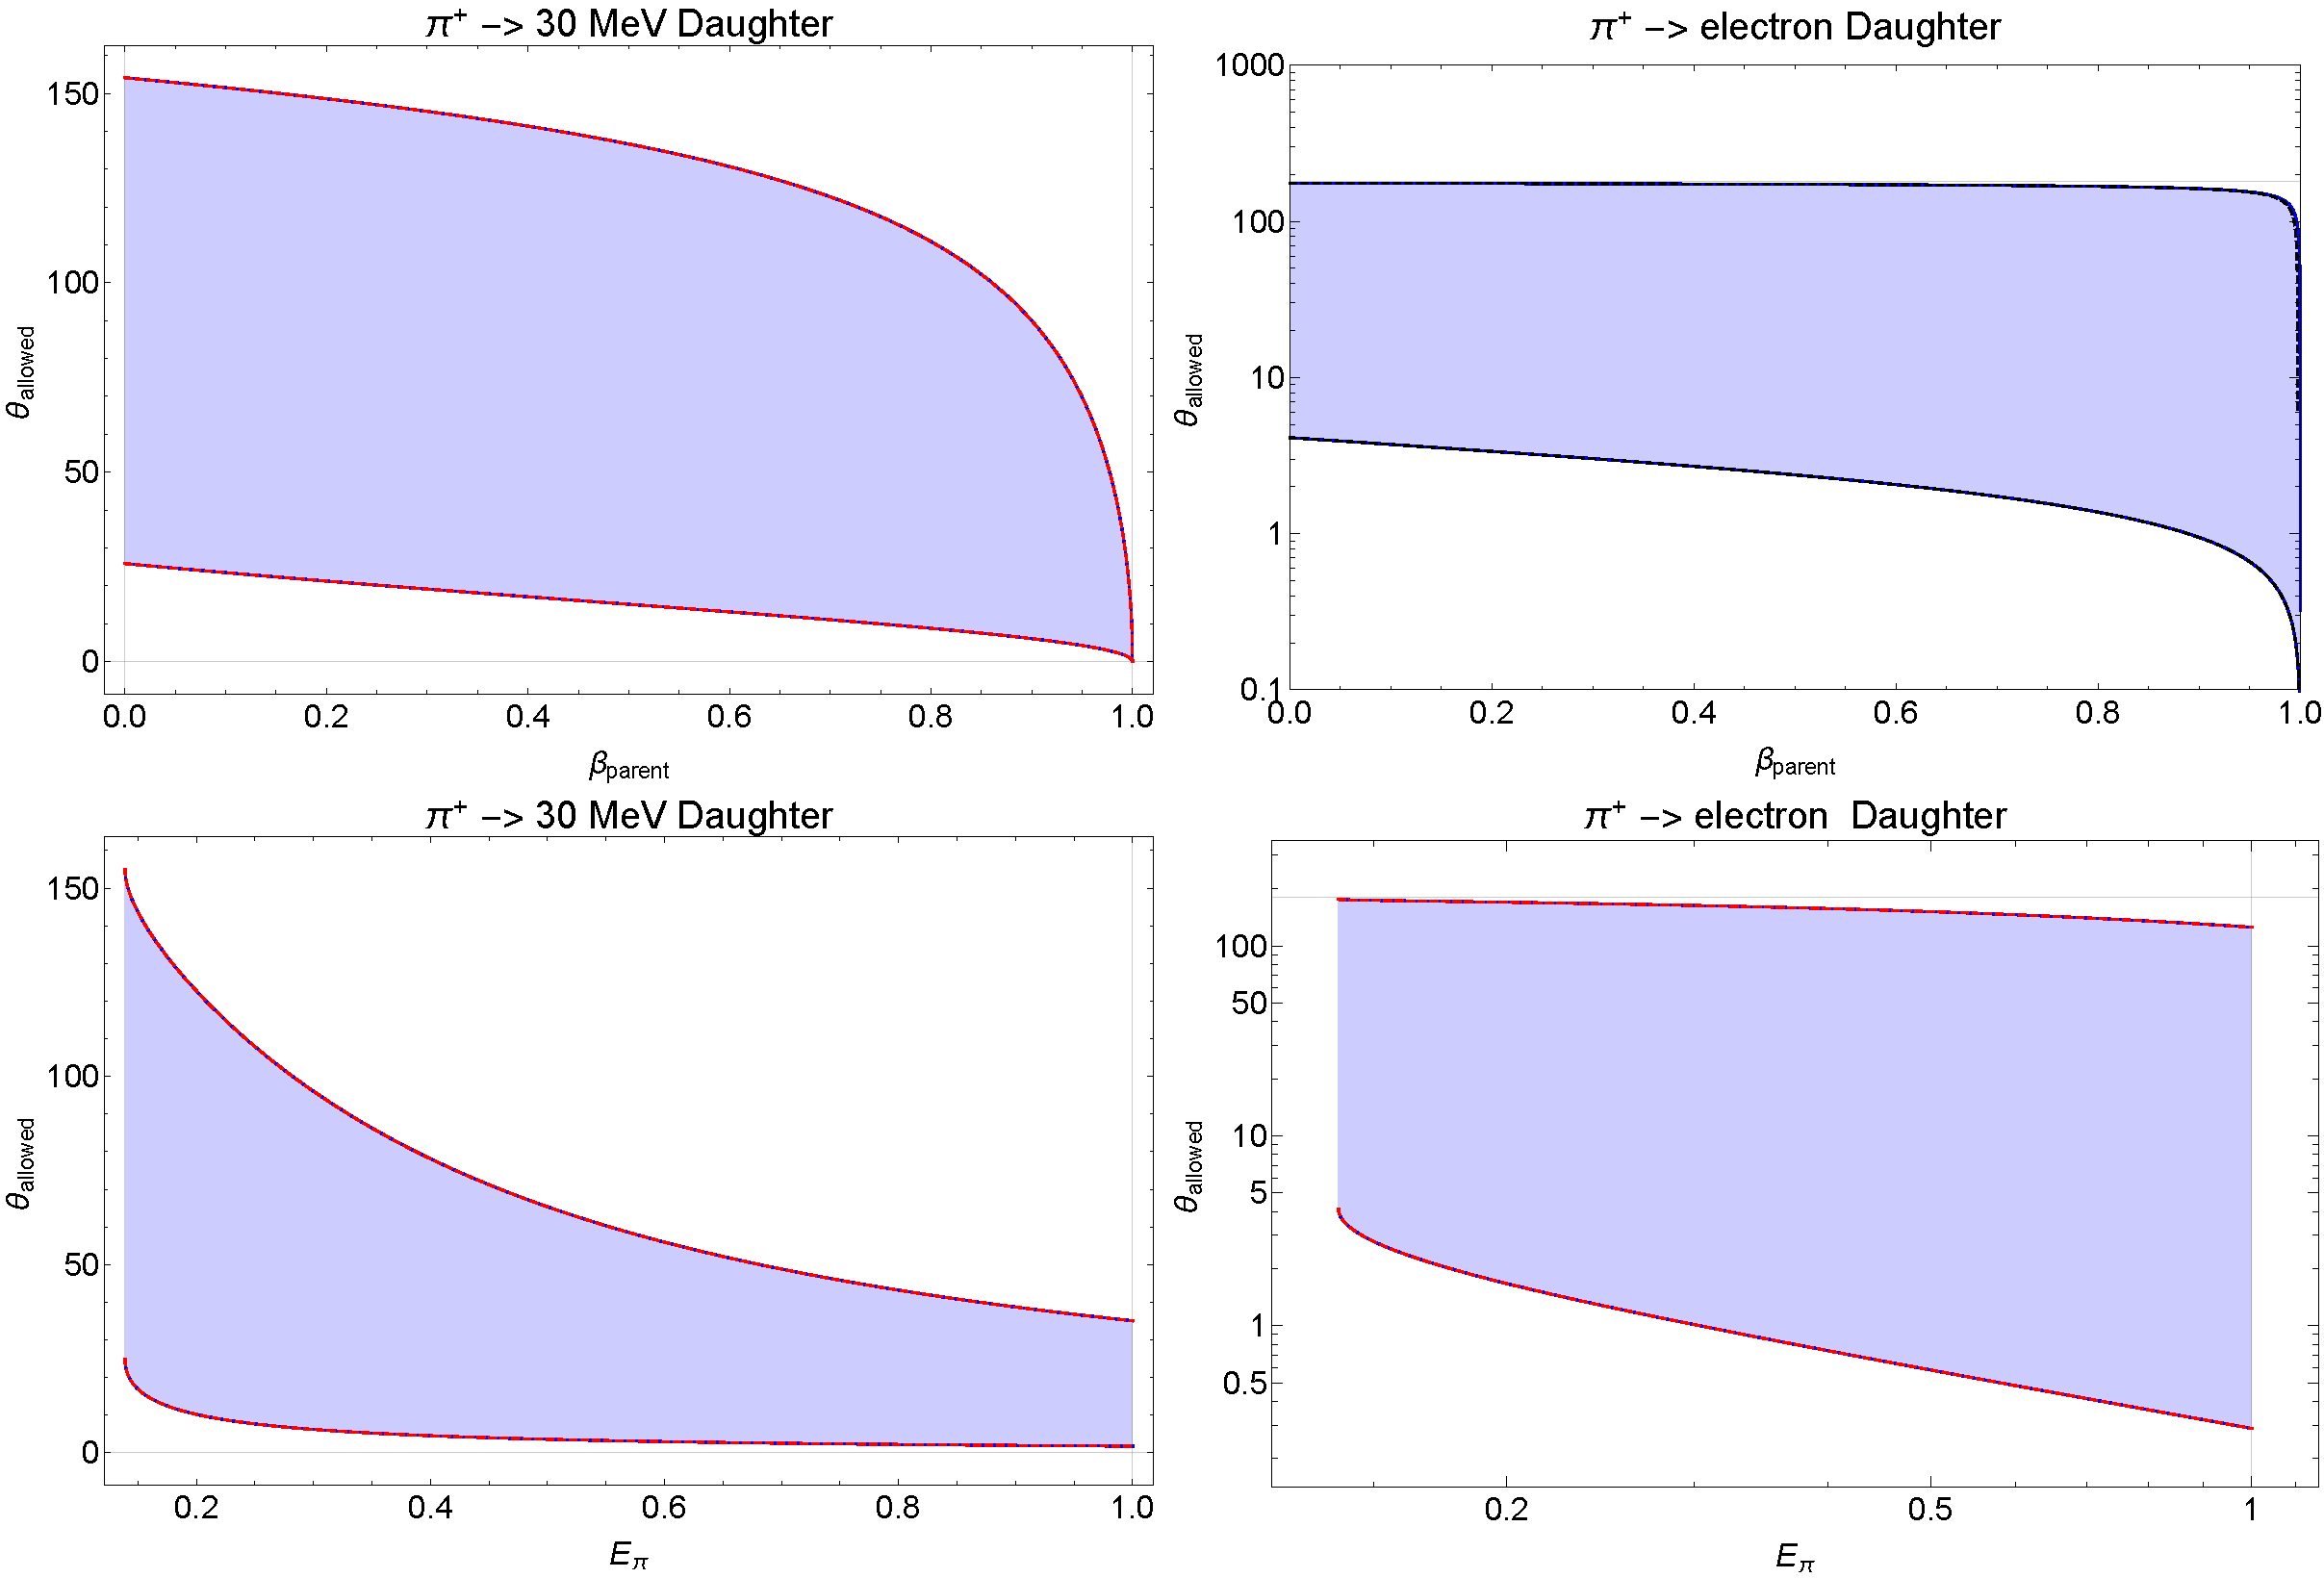
\includegraphics[width=1.0\textwidth]{figures/angles_boost.pdf}
\caption{\label{fig:boost} Allowed angles in the decay $m_\pi \rightarrow a+b$ for $m_a 30$ MeV and $m_a=m_e$. In the limit of $m_a \rightarrow 0$ the entire $\beta_\pi - \theta_a$ plane is covered, which is pretty much what we were calculating today!   .}
\end{figure}


\begin{figure}[t]
\center
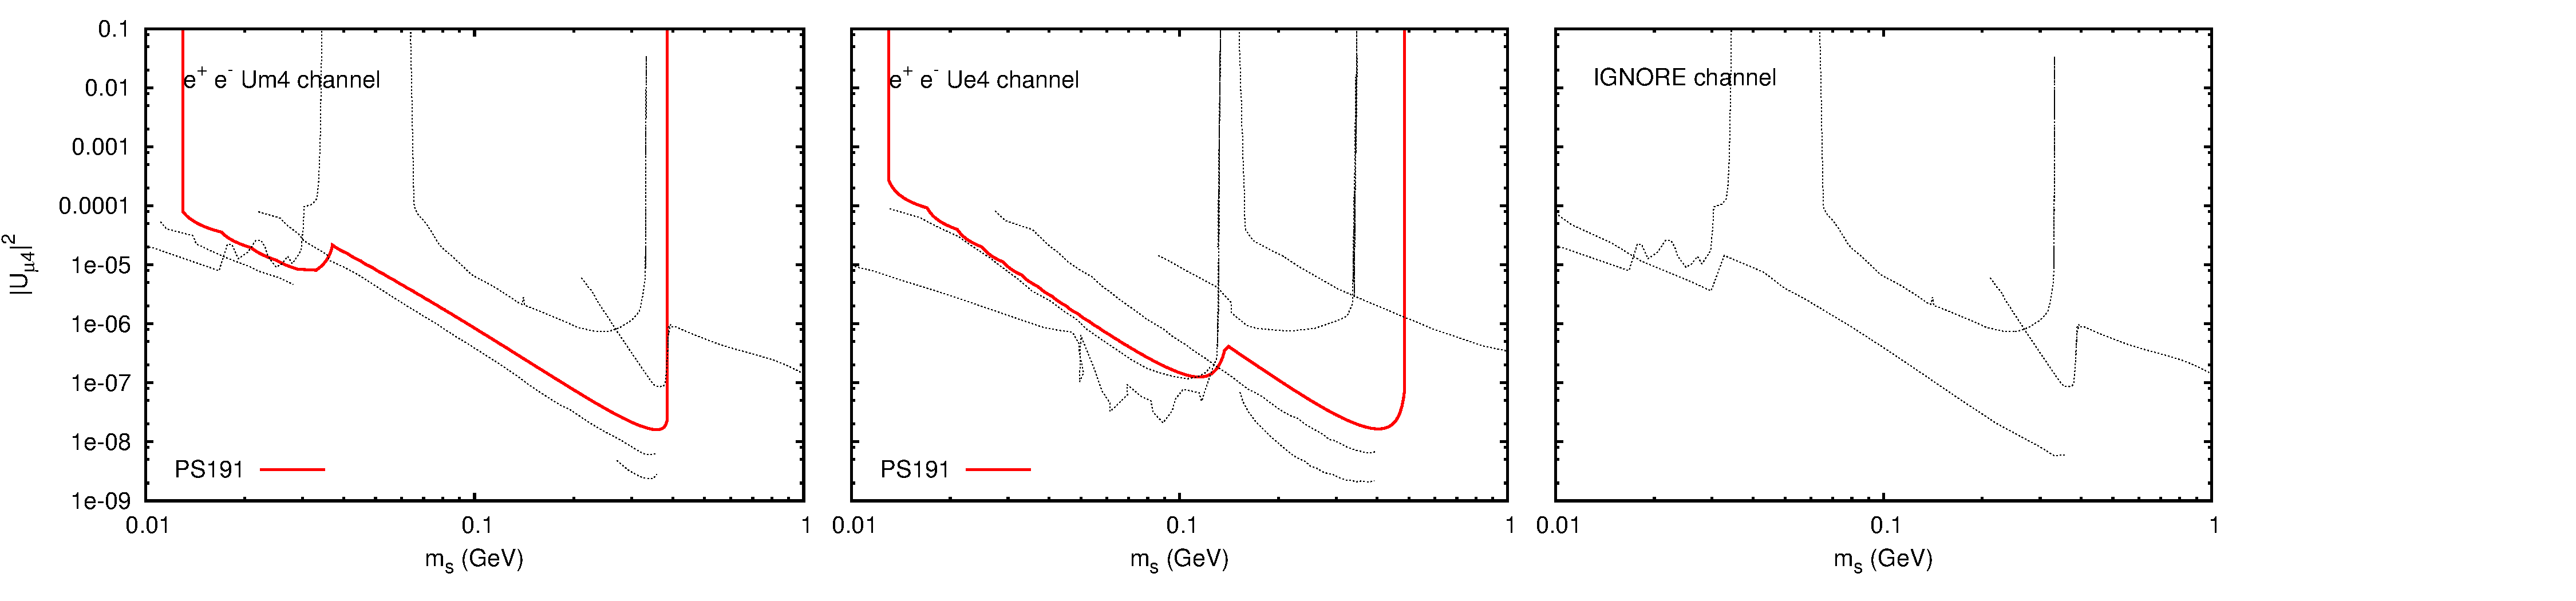
\includegraphics[width=1.0\textwidth]{figures/zerobg_um4_ps191_test.pdf}
\caption{The results of a PS191 run test, flux less certain.}
\end{figure}

	
\begin{figure}[t]
\center
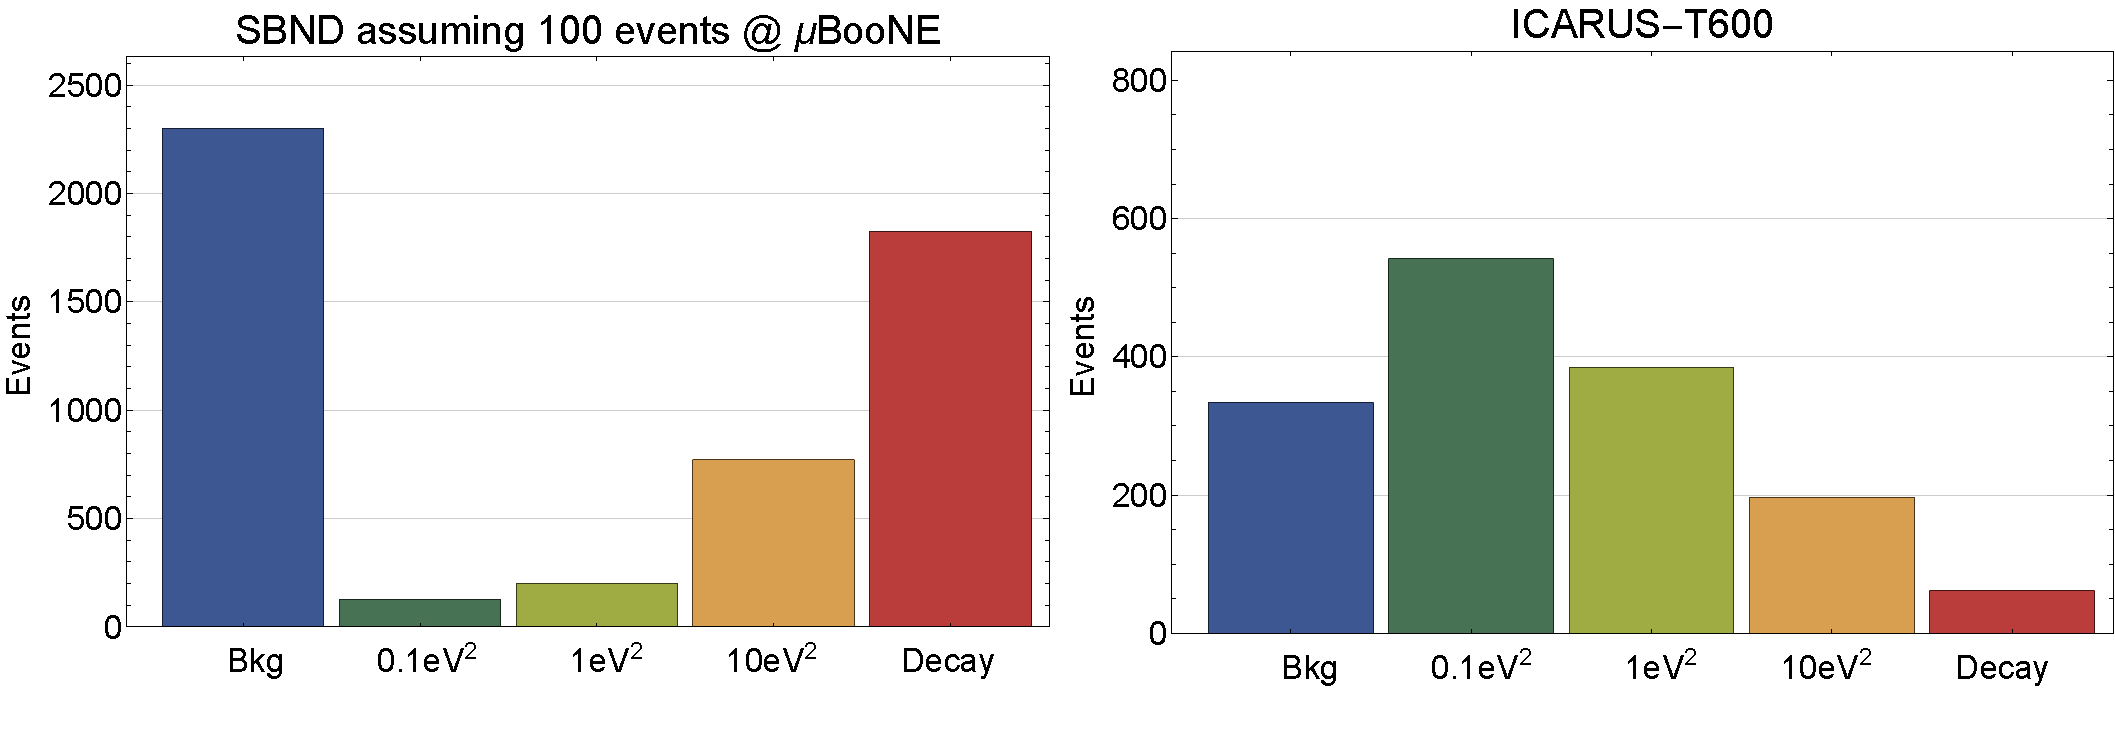
\includegraphics[width=0.7\textwidth]{figures/baseline_comp.pdf}
\caption{\label{fig:baseline_comp} Assuming MicroBooNE sees 100 events excess, what would SBND and ICARUS see if the 100 events was truely a background event, an oscillating sterile of 0.1 $\text{eV}^2$, 1  $\text{eV}^2$ or 10 $\text{eV}^2$ or a decaying 100 MeV sterile n flight. }
\end{figure}


%%%%%%%%%%%%%%%%%%%%%%%%%%%%%%%%
%%%%%%%%%%%%%%%%%%%%%%%%%%%%%%%%
%%%%%%%%%%%%%%%%%%%%%%%%%%%%%%%%

\bibliographystyle{apsrev4-1}
\bibliography{lib}{}

\end{document}

